\documentclass[12pt,reqno]{amsart}
\usepackage[margin = 1.3 in]{geometry}
%\usepackage[frenchmath,defaultmathsizes]{mathastext}
\usepackage{cite}
\usepackage{
  hyperref,
  amsmath,
  amssymb,
  tikz,
  amsthm,
  thmtools,
  microtype,
  stmaryrd,
  tikz-cd,
  mathrsfs,
  pgfplots
}
\usepackage{graphicx}
\usepackage[shortlabels]{enumitem}
\usepackage{import}
\usepackage{xifthen}
\usepackage{pdfpages}
\usepackage{transparent}
\usepackage{booktabs}
\usepackage{subcaption}

%\usepackage{showlabels}

\linespread{1.1}
\usepackage[all]{xy}
\usepackage{eucal}

\title{A universal formula for counting cubic surfaces}
\author{Anand Deopurkar, Anand Patel
  \& Dennis Tseng}

\dedicatory{Dedicated to our teacher, Joe Harris, on the occasion of
  his $70$th birthday.}



%-----------------------------------------------
\def\labelitemi{--}
\newcommand{\todo}[1]{\fbox{ToDo: #1}}
\renewcommand{\k}{k}
\DeclareMathOperator{\id}{id}
\DeclareMathOperator{\Bl}{Bl}
\DeclareMathOperator{\Orb}{\overline{Orb}}
\DeclareMathOperator{\Polar}{Polar}
\DeclareMathOperator{\res}{Res}
\DeclareMathOperator{\Pole}{Pole}
\DeclareMathOperator{\Hilb}{Hilb}
\DeclareMathOperator{\Sing}{Sing}
\DeclareMathOperator{\M}{\mathcal{M}}
\renewcommand{\to}{{\longrightarrow}}

\renewcommand{\sectionautorefname}{\S}
\renewcommand{\subsectionautorefname}{\S}
% Let us keep this minimial
% Let us also define things only if they are previously undefined.

% Common theorem-like environments
\ifcsname theorem\endcsname{}\else\declaretheorem[parent=subsection]{theorem}\fi
\ifcsname corollary\endcsname{}\else\declaretheorem[sibling=theorem]{corollary}\fi
\ifcsname lemma\endcsname{}\else\declaretheorem[sibling=theorem]{lemma}\fi
\ifcsname proposition\endcsname{}\else\declaretheorem[sibling=theorem]{proposition}\fi
\ifcsname conjecture\endcsname{}\else\declaretheorem[sibling=theorem]{conjecture}\fi
\ifcsname problem\endcsname{}\else\declaretheorem[sibling=theorem]{problem}\fi
\ifcsname question\endcsname{}\else\declaretheorem[sibling=theorem]{question}\fi
\ifcsname definition\endcsname{}\else\declaretheorem[sibling=theorem, style=definition]{definition}\fi
\ifcsname exercise\endcsname{}\else\declaretheorem[sibling=theorem, style=definition]{exercise}\fi
\ifcsname example\endcsname{}\else\declaretheorem[sibling=theorem, style=definition]{example}\fi
\ifcsname remark\endcsname{}\declaretheorem[sibling=theorem, style=remark]{remark}\fi

% Common abbreviations

% Absolutely standard rings and fields
\providecommand {\N}{{\bf N}}
\providecommand {\Z}{{\bf Z}}
\providecommand {\Q}{{\bf Q}}
\providecommand {\R}{{\bf R}}
\providecommand {\C}{{\bf C}}

% Common spaces grassmannian
\renewcommand {\P}{{\bf P}}
\providecommand {\Gr}{{\bf Gr}}
\providecommand {\A}{{\bf A}}

% Groups
\providecommand{\SL}{\operatorname{SL}}
\providecommand{\GL}{\operatorname{GL}}
\providecommand{\PGL}{\operatorname{PGL}}
\providecommand{\Gm}{{\bf G}_m}

% f \from G \to H reads much better than f \colon G \to H
\providecommand {\from}{{\colon}}

% Absolutely standard notation
\providecommand{\spec}{\operatorname{Spec}}
\providecommand{\proj}{\operatorname{Proj}}
\providecommand{\coker}{\operatorname{coker}}
% Kernel is already defined
\providecommand{\Blowup}{\operatorname{Bl}}
\providecommand{\Hom}{\operatorname{Hom}}
\providecommand{\Ext}{\operatorname{Ext}}
\providecommand{\Tor}{\operatorname{Tor}}
\providecommand{\End}{\operatorname{End}}
\providecommand{\Aut}{\operatorname{Aut}}
\providecommand{\codim}{\operatorname{codim}}
% Dim is already defined
\providecommand{\Pic}{\operatorname{Pic}}
\providecommand{\Sym}{\operatorname{Sym}}
\providecommand{\rk}{\operatorname{rk}}
\declaretheorem[sibling=theorem,style=remark]{remark}
\numberwithin{equation}{section}
\declaretheorem[title=Theorem]{maintheorem}
\renewcommand{\themaintheorem}{\Alph{maintheorem}}


\renewcommand{\O}{\mathcal O}
\newcommand{\G}{\mathbf G}
\newcommand{\F}{\mathbf F}
\newcommand{\td}{\widetilde}
\newcommand{\V}{\mathcal V}
\newcommand{\cP}{\mathcal P}
\newcommand{\cC}{\mathcal{C}}
\newcommand{\cX}{\mathcal{X}}
\newcommand{\hL}{\widehat{\mathcal{L}}}
\newcommand{\hpsi}{\widehat{\psi}}
\newcommand{\fm}{\mathfrak m}
\newcommand{\smvee}{\raise0.5ex\hbox{$\scriptscriptstyle\vee$}}
\newcommand{\hM}{\widehat{\M}}
\newcommand{\compl}[1]{\widehat{#1}}
\newcommand{\Spec}{{\text{\rm Spec}\,}}
\newcommand{\Spf}{{\text{\rm Spf}\,}}
\renewcommand {\o}[1]{\overline{#1}}
\newcommand{\Proj}{{\text{\rm Proj}\,}}
\newcommand{\git}{\sslash}
% -----------------------------------------------

%%% BEGIN DOCUMENT


\begin{document}

\maketitle

\begin{abstract}
  Using equivariant geometry, we find a universal formula that computes the number of times a general cubic surface arises in a family.
  As applications, we show that the $\PGL_4$ orbit closure of a generic cubic surface has degree 96120, and that a general cubic surface arises 42120 times as a hyperplane section of a general cubic 3-fold.
\end{abstract}




\section{Introduction}
\label{sec:intro}

Cubic surfaces have fascinated us for centuries. Ever since Cayley and
Salmon discovered the 27 lines, it has become somewhat of a tradition
to revisit their geometry, using increasingly sophisticated tools to
uncover more and more. Our contribution to this story provides a
universal answer to a collection of natural enumerative questions
about families of cubic surfaces.

The isomorphism classes of cubic surfaces form a 4-dimensional moduli
space. So, we expect that in a 4-dimensional family, a general
isomorphism class would appear finitely many times. How can we
determine this number? For example, how many times does a general
cubic surface appear, up to isomorphism, as
\begin{enumerate}[(A)]
\item \label{orbit} a member of a 4-dimensional general linear system of cubic surfaces in $\P^3$?
\item \label{slice} a hyperplane section of a general cubic threefold in $\P^4$?
\item a blow up of 6 points in $\P^2$ varying in a general
  4-dimensional linear system on a cubic curve?
\end{enumerate}
Our formula answers all questions of this kind.  The answers to these
specific questions are $96120$, $42120$, and $25920$, respectively.

To state our formula, we must fix a precise moduli space of cubics.
Let us denote by $\mathcal M$ the GIT quotient of the set of
semi-stable cubic surfaces in $\P^3$ by the action of $\PGL_4$.  By a
\emph{family of cubic surfaces}, we mean a flat, proper morphism whose
geometric fibers are isomorphic to cubic surfaces in $\P^3$.

\begin{theorem}\label{theorem:main}
  Let $\pi \colon \cX \to B$ be a good family of cubic surfaces over a
  proper base $B$, let $\V$ denote the rank 4 vector bundle
  $ \pi_* \left(\omega_\pi^{-1}\right)$, and let
  \(v_i = c_i\left(\V\right)\) be its Chern classes.  Assume that a
  general fiber of $\pi$ is semi-stable, and let
  $\mu \colon B \dashrightarrow \mathcal M$ be the induced moduli map.  Then,
  \begin{align}
    \deg \mu =
    \label{eq:MAIN}
    1080 \int_{B} \left(v_{1}^{2}v_{2} - v_{1}v_{3}+ 9v_{4}\right).
  \end{align}
\end{theorem}
\autoref{def:goodfamily} gives the precise meaning of a ``good''
family.  This notion includes any family whose fibers are
GIT-semi-stable or have a finite automorphism group.

\subsection{Degree of the orbit closure}
Question~\ref{orbit} in \autoref{sec:intro} fits in a broader story
that has been an ongoing topic of study.  Consider a hypersurface
\(X\) in a projective space $\P V$ cut out by a homogeneous polynomial
$F \in \Sym^d V^\vee$.  In $\P\Sym^dV^\vee$, consider the orbit of
$[F]$ under the action of $\GL(V)$, and let $\Orb([F])$ be its
closure.  To our knowledge, this story begins in 1897 with Enriques
and Fano, who computed the degree of the orbit closure of simple
binary forms of all degrees \cite{enriques.fano:97}.  In a series of
seminal papers, Aluffi and Faber computed the degree of the orbit
closure for \emph{all} binary and ternary forms.  That is, the case of
points in $\P^1$ and curves in $\P^2$ has been done.  The next case is
that of a general cubic surface in $\P^3$, which we do in this paper.
\autoref{theorem:main} applied to Question~\ref{orbit} says that the
degree of the orbit closure of a general cubic surface is $96120$.

Question~\ref{orbit} appears as one of the ``twenty-seven questions
about the cubic surface'' by Ranestad and Sturmfels \cite{ran.stu:20}.
In 2019, Brustenga i Moncus\'i, Timme, and Weinstein gave a
``numerical proof'' for the number 96120. In 2020, Cazzador and
Skauli outlined an approach towards a proof by following the
techniques of Aluffi and Faber \cite{bru-i-mon.tim.wei:20,caz.ska:20}.
Our approach is different.

\subsection{The equivariant class of the orbit closure}
Our key idea is to consider not just the degree of the orbit closure,
but the class of the orbit closure in the equivariant Chow ring
$A^\bullet_{\GL V}(\Sym^dV^\vee)$. Although the equivariant class subsumes the
degree, finding it turns out to be easier than finding the degree.

Let us explain how the equivariant class yields the degree.
We have natural maps
\[
\begin{tikzcd}
  A^\bullet_{\GL V}(\Sym^dV^\vee) \ar{r}& A^\bullet_{\GL V}(\Sym^d V^\vee \setminus
  \{0\}) \otimes \Q \ar[equal]{d}\\
  &A^\bullet_{\PGL V}(\P \Sym^dV^\vee) \otimes \Q \ar{r}&
  A^\bullet(\P \Sym^dV^\vee) \otimes \Q.
\end{tikzcd}
\]
Under the composite map, the class of $\Orb(F) \in A^\bullet_{\GL
  V}(\Sym^dV^\vee)$ is mapped to the class of $\Orb([F]) \in
A^\bullet(\P \Sym^dV^\vee) \otimes \Q$, which is simply the degree of $\Orb([F])$.

Let us explain what makes it possible to find the equivariant
class.  The ring $A^\bullet_{\GL V}(\Sym^dV^\vee)$ is the polynomial ring
in variables $c_1, \dots, c_r$, where $r = \dim V$, and the variable
$c_i$ has degree $i$.  The equivariant class of $\Orb(F)$ lies in the
graded component $A^m(\Sym^dV^\vee)$, where
$m = \dim \Sym^d V^\vee - \dim \GL V$.  As a result, it can be expressed as
a $\Z$-linear combination of monomials in $c_i$ of total degree
$m$. We can now use the method of undetermined coefficients.  We
construct maps $B \to [\Sym^dV^\vee/\GL V]$ where the pull-back of
$\Orb(F)$ as well as the classes $c_i$ can be explicitly
computed. Every such family gives a linear relationship between the
coefficients in the expression of $\Orb(F)$, which are to be determined.
If we have enough families, we get enough information to find all the coefficients.
For cubic surfaces, we construct more than enough families---there are 5
coefficients to be determined and we construct 8 families. The redundancy
serves as an extra check on the result.
\begin{theorem}\label{thm:eqvclass2}
  Let $V$ be a 4-dimensional vector space and let $F$ be a general
  element of $\Sym^3 V^\vee$.
  The equivariant class of the $\GL(V)$-orbit closure $\Orb(F)$ of $F$
  in $A^\bullet_{\GL V}(\Sym^3 V^\vee)$ is given by
  \[
    [\Orb F] = 24c_1^4 + 12c_1^2c_2 - 6c_1c_3 + 9c_4,
  \]
  where the \(c_i = c_i(V)\) are the Chern classes of the tautological vector
  bundle $V$.
\end{theorem}
The formula in \autoref{thm:eqvclass2} appears to be different from the one
in \autoref{theorem:main}, but they are related by a simple change of
variables; see \autoref{proof:eqvclass2}.

Most of the paper is devoted to constructing {\sl provably} good
families of cubic surfaces on which we can compute $\deg \mu$ and the
Chern classes $c_i$.  Proofs of goodness are sometimes challenging --
this is one instance of the general problem of determining which
homogeneous forms lie in the $GL$-orbit closure of which other forms.
For us, a particularly difficult case was to show that the $A5$ cubic
$V(x_0 x_1 x_3 - (x_0^3 + x_1^3 - x_1x_{2}^2))$ is not in the closure
of a general orbit, and this task occupies the entire appendix. To give a teaser for our test families, we list their
bases $B$ here: $\P^4$, $\overline M_{0,7}$, a
Hassett-weighted variant of $\overline M_{0,7}$, a blow up of the
Hilbert scheme of two points on a quintic del Pezzo surface, and last
but not least, the stack $B\G_m$.

The method of undetermined coefficients applies to hypersurfaces of
any degree and dimension.  The obstacle, in general, is in
constructing enough families.  Our constructions crucially use the
beautiful geometry of the lines on a cubic, and therefore are very
specific to the cubic surface case.

\subsection{Further remarks}
The formula in \autoref{theorem:main} has some curious consequences.
\begin{corollary}
  \label{cor:ineq} If $\pi \colon \cX \to B$ is a good family of cubic
  surfaces parametrized by a $4$ dimensional proper variety $B$,
  then $$\int_{B} v_{1}^{2}v_{2} - v_{1}v_3 + 9v_{4} \geq 0$$ with
  equality holding if and only if a general cubic surface does not
  arise as a fiber.
\end{corollary}

\begin{corollary}
  \label{cor:ineq} Let $\pi \colon \cX \to B$ is a good family of cubic
  surfaces parametrized by a $4$ dimensional proper variety $B$.
  Assume that a general fiber of $\pi$ is smooth and the induced map
  $\mu \colon B \dashrightarrow \mathcal M$ is dominant.
  Then the degree of $\mu$ is divisible by 1080.
\end{corollary}
In particular, a parameter space for cubic surfaces that carries a
good universal family must cover $\mathcal M$ by a map of degree
divisible by 1080.  Interestingly, the number 1080 is also the least
common multiple of the orders of the finite groups that arise as
automorphism groups of cubic surfaces.
We wonder if $1080$ is the minimal positive integer realizable as $\deg \mu$ as we vary
across all good families of cubic surfaces.

\subsection{Future directions}

\autoref{thm:eqvclass2} is only the beginning.  Each {\sl particular}
cubic surface $F=0$ registers its own equivariant orbit class
$[\Orb(F)]$.  A refined study of the methods developed in this paper
may afford us a complete understanding of how this class changes
according to special changes in the geometry of $F=0$, e.g. acquiring
singularities or Eckhart points.  This is something we hope to pursue
in the future.

In a different direction, there should be analogous formulas counting
Del Pezzo surfaces of degrees $1,2$ and $4$.  We fully expect our
methods to establish formulas in these settings, though we have not
even begun the analysis.  



\subsection{Acknowledgements}
We thank Radu Laza, who asked Question~\ref{slice} to the first two
authors during a meeting at Oberwolfach in the summer of 2016.  We
thank Hunter Spink for important discussions during the infancy
of the project.  We thank Paolo Aluffi for quickly providing an
enumerative reference on cuspidal cubic curves and Jarod Alper for discussions on equivariant geometry.



  


%---------------------------------------------------------------------------


\section{Preliminaries}
\label{sec:good}

In this chapter, we introduce the notion of a good family of cubic
surfaces (\autoref{def:goodfamily}) and provide a tool
(\autoref{prop:good}) to verify that a family is good.  Before we do
so, we first establish notation and recall some facts about cubic surfaces and their moduli.
\subsection{Notation and conventions}
\label{sec:notation-conventions}
Fix an algebraically closed field $\k$ of characteristic zero.  In
this paper, a `scheme' means `a scheme of finite type over $\k$' and a
`point' means a `$\k$-point', unless explicitly stated otherwise.  We
do not distinguish between a vector bundle and the associated locally
free sheaf of its sections.

Given a map of schemes $\pi \colon X \to Y$ and a point $y \in Y$, we
let $X_y$ denote the fiber scheme $\pi^{-1}(y)$.  If $\pi$ is proper
and Gorenstein, we write $\omega_{X/Y}$ or $\omega_\pi$ for the
dualizing line bundle.  If $X$ and $Y$ are themselves Gorenstein and
$\pi$ is flat, then we have
$\omega_{X/Y} = \omega_X \otimes \pi^*\omega_Y^{-1}$.

Given a vector bundle $\mathcal W$, we let $\P \mathcal W$ be its
projectivization.  Contrary to Grothendieck's convention,
$\P \mathcal W$ parametrizes $1$-dimensional subspaces in the fibers
of $\mathcal W$.  In other words, we set
\[ \P \mathcal W = \Proj \Sym(\mathcal W^\vee).\] As a result,
$\P \mathcal W$ comes equipped with a line bundle $\O(1)$ whose
push-forward to the base is $\mathcal W^\vee$.

Let $Q \subset \P V$ be a non-degenerate quadric.  The bilinear form
associated to $Q$ gives an isomorphism of $\P V$ with the dual
projective space $\P V^\vee$.  Given a point $p \in \P V$, we denote
by $\Polar_Q(p) \subset \P V$ the hyperplane dual to $p$ with respect to
$Q$. Similarly, given a hyperplane $H \subset \P V$, we denote by
$\Pole(H) \in \P V$ the point dual to $H$ with respect to $Q$.  In
almost all cases, we use these constructions when $\P V$ is $\P^2$.

\subsection{Moduli of cubic surfaces}
\label{sec:classical-facts}
Let $\pi \colon \cX \to B$ be a family of cubic surfaces.  That is,
let $\pi$ be a flat, proper morphism whose fibers are isomorphic to
cubic hypersurfaces in $\P^3$.  Since $\pi$ is flat and its fibers are
Gorenstein, it is a Gorenstein morphism, and hence admits a dualizing
line bundle $\omega_\pi$.  By the adjunction formula, it follows that
the restriction of $\omega_{\pi}^{-1}$ to every fiber is isomorphic to
the restriction of $\O(1)$ with respect to an embedding of the fiber
as a cubic hypersurface in $\P^3$.  By standard theorems about
cohomology and base-change, it follows that
$R^i\pi_* \left(\omega_{\pi}^{-1}\right)$ vanishes for $i > 0$, and is
a vector bundle for $i = 0$.  Set
\[ \mathcal V = \pi_* \left( \omega_\pi^{-1} \right).\]
The natural map 
\[ \pi^*\mathcal V \to \omega_{\pi}^{-1}\]
yields a closed embedding
\begin{equation}\label{eqn:relcanx}
  \cX \subset \P \mathcal V^\vee.
\end{equation}
We know that
\[ \omega_{\P \mathcal V^\vee/B} = \O(-4) \otimes \det \mathcal V^\vee,\]
and hence, by adjunction,
\[ \omega_{\cX/B}= \O(-4) \otimes \O(\cX) \otimes \det \mathcal V^\vee |_\cX.\]
By construction, we also have
\[ \omega_{\cX/B} = \O(-1)|_\cX,\]
and hence we obtain that
\begin{equation}\label{eqn:ox}
  \O(\cX) = \O(3) \otimes \det \mathcal V.
\end{equation}
In other words, $\cX \subset \P \mathcal V^\vee$ is the zero locus of
a section of the line bundle $\O(3) \otimes \det \mathcal V^\vee$.

Consider the category $\mathscr {C}$ fibered in groupoids over the
category of schemes whose objects over a scheme $B$ are families of
cubic surfaces $\pi \colon \cX \to B$, and whose morphisms are pull-back
diagrams.  Consider the category $\mathscr {M}$ fibered in groupoids
over the category of schemes whose objects over a scheme $B$ are
vector bundles $\mathcal V$ over $B$ of rank 4 along with a nowhere
zero section $\xi$ of
$\Sym^3 \mathcal V^\vee \otimes \det \mathcal V$, and whose morphisms
are pull-back diagrams.  Let $V$ be a $\k$-vector space of dimension
4.  Note that $\mathscr{M}$ is simply the quotient stack
\[\mathscr{M} = \left[\Sym^3 V^\vee \otimes \det V \setminus \{0\} / \GL V \right]. \]
\begin{proposition}\label{prop:cubicstack}
  The category $\mathscr{C}$ of families of cubic surfaces is equivalent to the category $\mathscr{M}$.
\end{proposition}
\begin{proof}
  Let $\pi \colon \cX \to B$ be a family of cubic surfaces, and set
  $\mathcal V = \pi_* \left( \omega_{\pi}^{-1} \right)$.  Consider the
  relative canonical embedding $\cX \subset \P \mathcal V^\vee$.  In
  this embedding, $\cX$ is cut out by a section of
  $\O(3) \otimes \det \mathcal V$ on $\P \mathcal V^\vee$, or
  equivalently, by a section of $\xi$ of
  $\Sym^3V^\vee \otimes \det \mathcal V$ on $B$.  Since $\pi$ is flat,
  $\xi$ is nowhere zero on $B$.  We thus have a natural transformation
  from $\mathscr{C}$ to $\mathscr{M}$.

  To go from $\mathscr{M}$ to $\mathscr{C}$, given a rank 4 bundle $\mathcal V$ and a nowhere section $\xi$ of $\Sym^3 \mathcal V^\vee \otimes \det \mathcal V$, define $\cX \subset \P \mathcal V^\vee$ as the zero-locus of the corresponding section of $\O(3) \otimes \det \mathcal V$.
\end{proof}

We call $\mathscr{M}$ the \emph{moduli stack of cubic surfaces}.
Sometimes, it will be convenient to add in the zero section and consider the bigger stack
\[ \mathscr{M}^* = \left[\Sym^3 V^\vee \otimes \det V / \GL V \right].\]
Note that the diagonal $\G_m \subset \GL V$ acts by weight $-1$ on $\Sym^3 V^\vee \otimes \det V$.
In particular, its action is free.
Therefore, the stack $\mathscr{M}$ is isomorphic to the quotient stack
\[ \mathscr{M} = \left[ \P \Sym^3V^\vee / \PGL V \right].\]

We let $\mathcal M$ denote the GIT quotient of $\P \Sym^3V^\vee$ by
the action of $\PGL V$.  The semi-stable and stable locus of the
action were computed by Mumford; see \cite[Chapter 4, \S
2]{mum.fog.kir:94} or \cite[1.14]{mum:77}.  The stable locus consists
of surfaces with at worst $A_1$ singularities, and the semi-stable
locus includes surfaces with at worst $A_2$ singularities.  The ring
of invariants was computed much earlier, in the 1860s, by Salmon
\cite{sal:60} and Clebsch \cite{cle:61,cle:61*1}, and later by
Beklemishev \cite{bek:82} using more modern methods.  The invariant
ring is freely generated by polynomials of degree 8, 16, 24, 32, and
40, and as a result, the coarse moduli space $\mathcal M$ is
isomorphic to the weighted projective space $\P(1,2,3,4,5)$.

We recall perhaps the most famous fact about cubic surfaces, discovered in 1849. 
\begin{theorem}[Cayley \cite{cay:49}, Salmon \cite{sal:49}]
  \label{theorem:cayleysalmon}
  Every smooth cubic surface contains exactly $27$ lines.
\end{theorem}
As we know, the 27 lines are key to understanding geometry of the
cubic surface.  Each line is a $(-1)$-curve, and hence contractible by
Castelnuovo's theorem.  A set of lines that are pairwise skew is
particularly important, because they can be blown down simultaneously.
The maximum number of such lines is 6, and they allow us to realize
the cubic surface as a blow up of $\P^2$ at 6 points.

Following Schl\"afli \cite{sch:58}, we call an ordered tuple of pairwise disjoint six lines $(\ell_1, \dots, \ell_6)$ on a cubic surface a \emph{six}.
A \emph{double six} is an unordered pair of sixes $\{(\ell_1, \dots, \ell_6), (\ell_1', \dots, \ell_6')\}$ such that
\begin{itemize}
\item $\ell_{i}$ and $\ell'_{i}$ are disjoint for all $i$, and
\item $\ell_{i}$ and $\ell'_{j}$ meet at a point whenever $i \neq j$.
\end{itemize}

\begin{theorem}[Schl\"{a}fli \cite{sch:58}]
  \label{theorem:schlafli} Each six on a smooth cubic surface has a unique extension to a double-six, and every smooth cubic surface contains $36$ double-sixes.
\end{theorem}
Thus, each smooth cubic surface admits 72 distinct maps to
$\P^2$, up to automorphisms of $\P^2$, each of which
blows down 6 lines.

The sixes on a cubic surface allow us to relate $\mathcal M$ to a more
familiar moduli space.  Let $\mathcal M^\dagger$ denote the moduli
space of pairs $(S, \ell)$, where $S$ is a smooth cubic surface and
$\ell$ is a six on $S$.  By \autoref{theorem:schlafli}, the natural
forgetful map
\begin{align*}
  \sigma \colon \mathcal M^\dagger &\to \mathcal M \\
  (S, \ell) &\mapsto S
\end{align*}
is dominant and quasi-finite of degree
\[ \deg \sigma = 72 \times 6! = 51840.\] On the other hand, the space
$\mathcal M^\dagger$ is isomorphic to the configuration space of 6
ordered points on $\P^2$
\[ \mathcal M^\dagger \xrightarrow{\sim} \left( (\P^2)^6 \setminus
    \text{Diagonals} \right) / \Aut(\P^2).\] The isomorphism sends
$(S, (\ell_i))$ to $(\P^2, (p_i))$, where $\beta \colon S \to \P^2$
blows down the lines $\ell_i$ and $p_i = \beta(\ell_i)$.

Finally, in our third test family we will need to use the following
enumerative fact, originally due to Schubert, about cuspidal cubic
curves---see the remarkable paper of Miret and Xamb\'o
\cite{miret1989geometry}.

 \begin{theorem}[Schubert, Miret, Xamb\'o]
   \label{theorem:Schubert} There are $20$ cuspidal cubic curves
   containing all of five general points in $\P^{2}$, and flexed at a
   sixth general point.
 \end{theorem}
\subsection{Equivariant Chow groups and equivariant orbits}
The standard reference for equivariant Chow theory is \cite{edi.gra:98}.
We recall a few relevant notions, mostly to set notation.

Given an algebraic space $X$ with an action of an algebraic group $G$,
denote by $A^i_G(X)$ the $G$-equivariant Chow group of codimension $i$
cycles.  Given a $G$-invariant subspace $Y \subset X$ of pure
codimension $i$, denote by $[Y] \in A^i_G(X)$ the fundamental class of
$Y$.  If $Y \subset X$ has codimension $> i$, then the restriction map
\[ A^i_G(X) \to A^i_G(X \setminus Y)\] A $G$-linearized vector bundle
$V$ on $X$ admits equivariant Chern classes $c_i(V) \in A^i_G(X)$.
The equivariant Chow groups are homotopy invariant: if $Y \to X$ is a
$G$-equivariant vector bundle, then the pull-back map
$A^i_G(X) \to A^i_G(Y)$ is an isomorphism.  If $X$ is smooth, then
$A^*_G(X)$ is a graded ring, where the multiplication is given by the
intersection product.

The $G$-equivariant Chow groups of $X$ are the same as the Chow groups
of the quotient stack $[X/G]$:
\[ A^i\left( [X/G] \right) = A^i_G(X).\]

The equivariant Chow ring of a point with the action of $G = \GL_n$ is
the polynomial ring
\[ A_{\GL_n}(\bullet) = \Z[c_1,\dots, c_n],\] where $c_i$ has
degree $i$ and can be identified with the $i$-th Chern class of the
standard $n$-dimensional representation of $\GL_n$.  By homotopy
invariance, for any $\GL_n$ representation $W$, we have
\[ A_{\GL_n}(W) = \Z[c_1,\dots,c_n].\] If the general linear
group under consideration is $\GL V$, where $V$ is a vector space,
then we write $v_i$ for the $i$-th Chern class of the tautological
representation $V$.  Then we have
\[ A_{\GL V}(W) = \Z[v_1,\dots,v_n].\]

Let $V$ be a $4$-dimensional $\k$-vector space.
Consider the $\GL V$ representation $W = \Sym^3 V^\vee \otimes \det V$.
By \autoref{prop:cubicstack}, (non-zero) $\GL V$ orbits in $W$ correspond canonically to cubic surfaces.
Note that the action of $\GL V$ on $W$ is generically free, and hence the codimension of a generic orbit is $20-16 = 4$.
Given a point $w \in W$, let $\Orb(w)$ denote the closure of its $\GL V$ orbit, and let
\[ [\Orb(w)] \in A^4_{\GL V}(W) = A^4(\mathscr M)\]
denote the fundamental class.
By a slight abuse of notation, if $X \subset \P^3$ is a cubic surface or $F \in k[X_0, \dots, X_3]$ is a non-zero cubic form, we let $\Orb(X)$ or $\Orb(F)$ denote the closure of the orbit in $W$ of the corresponding point $w$, and $[\Orb(X)]$ or $\Orb(F)$ the fundamental class.
Since $\A^4(\mathscr M)$ is generated by monomials in the Chern classes $c_i$ of total degree 4, we have an expression
\begin{equation}\label{eqn:chernexpansion}
  [\Orb(X)] = a_{1^4}v_1^4 + a_{1^2\cdot 2} v_1^2v_2 + a_{1\cdot 3} v_1v_3 + a_{2^2}v_2^2 + a_4 v_4,
\end{equation}
where the coefficients $a_i$ are integers.
The coefficients \eqref{eqn:chernexpansion} depend on $X$, but it is easy to argue that they remain constant as $X$ varies in a non-empty Zariski open subset of the space of cubic surfaces.

We let
\[ \partial \Orb(X) = \Orb(X) \setminus \GL V \cdot X,\]
denote the boundary of the orbit closure.
Note that $\partial \Orb(X) \subset W$ has codimension greater than $5$.

\subsection{Good families}
\label{sec:good-families}
Our strategy is to compute $[\Orb(X)]$ for a generic $X$ by pulling it back to various families $B \to \mathscr M$.
If there is a point of $B$ that lies in every $\Orb(X)$, then we have the issue of excess intersection. 
A good family is one that does not suffer from this defect.
Recall that $V$ is a $4$-dimensional $\k$-vector space.
\begin{definition}[Good family]
\label{def:goodfamily}
A family of cubic surfaces $\pi \colon \cX \to B$ is \emph{good} if
the following holds: there exists a non-empty Zariski open subset
$U \subset \Sym^3V^\vee$ such that for every $F \in U$ and $b \in B$,
the fiber $\cX_b$ does not lie in $\partial \Orb(F)$.
\end{definition}
\begin{example}[Fibers with finite automorphism groups]
  \label{ex:finaut}
  Suppose every $\cX_b$ has a finite automorphism group.  Then
  $\pi \colon \cX \to B$ is good.  Indeed, let $U$ be the subset
  consisting of elements with finite automorphism group.  For every
  $F \in U$, the boundary $\partial \Orb(F)$ consists of elements with
  a positive dimensional automorphism group, and hence it cannot
  contain $\cX_b$.
\end{example}
\begin{example}[GIT semistable fibers]
  \label{ex:semistable}
  Suppose every fiber $\cX_b$ is GIT-semistable.
  Then the family $\pi \colon \cX \to B$ is good.
  Indeed, let $U$ be the subset consisting of GIT-stable elements.
  For every $F \in U$, the orbit of $F$ is closed in the semi-stable locus, and hence $\partial \Orb(F)$ cannot contain $\cX_b$.
\end{example}

\begin{proposition}\label{prop:goodisgood}
  Let $\pi \colon \cX \to B$ be a good family of cubic surfaces.
  Assume that $B$ is proper of dimension 4 and a general fiber $\cX_b$ is semi-stable.
  Let $\mu \colon B \to \mathscr M$ be the map induced by $\pi$ and $m \colon B \dashrightarrow \mathcal M$ the rational map to the coarse moduli space.
  Then
  \[ \deg m = \deg \mu^*\left( \Orb(F) \right)\]
  for a general cubic form $F$.
\end{proposition}
\begin{proof}
  There exists an open $W \subset \mathcal M$ such that $m^{-1} (W) \to W$ is a finite \'etale morphism.
  Then the degree of $m$ is simply the number of points in $m^{-1}(u)$ for $u \in W$.
  By shrinking $W$ if necessary, we may assume that the map
  \[ \mathscr M^{ss} \to \mathcal M\]
  is an isomorphism over $W$.

  Let $U$ be as in the definition a good family.
  Then, for every $u \in U$, we have the equality
  \[ \cX \times_{\mathscr M} u = \cX \times_{\mathscr M} \overline u.\]
  By shrinking $U$ if necessary, we may assume that $U$ consists of semi-stable points and maps to $W \subset \mathcal M$ in the coarse space.
  Then, for every $u \in U$, we have
  \begin{align*}
    \deg \mu^* \Orb(u) &= \# \left(\cX \times_{\mathscr M} u \right)\\
                       &= \# \left(\cX \times_{\mathcal M} u\right) \\
                       &= \deg m.
  \end{align*}
\end{proof}

\subsection{Cubic surfaces as blow-ups}
Cubic surfaces arise as blow ups of $\P^2$ at six points, or more generally, as blow ups of del Pezzo surfaces of degree $d$ in $(d-3)$ points.
Varying the center of blow up is a convenient source of families of cubic surfaces.
The following proposition identifies certain nice sub-schemes to blow up.

\begin{definition}[Admissible subscheme]
  \label{def:admissible}
  Let $S$ be a smooth del Pezzo surface of degree $d \geq 3$ and let $Z \subset S$ be a subscheme of length $(d-3)$.
  We say that $Z$ is \emph{admissible} if 
  \begin{enumerate}
  \item $Z$ is curvilinear (contained in a smooth curve),
  \item $h^{0}\left(\mathcal{I}_Z \otimes \omega_S^{-1}\right) = 4$, and
  \item $\mathcal I_Z \otimes \omega_S^{-1}$ is generated by its global sections.
  \end{enumerate}
\end{definition}
The last condition means that $Z$ is scheme-theoretically cut out by the sections of $\omega_S^{-1}$ that vanish on it.

\begin{proposition}
  \label{prop:admissibleblowup}
Let $Z \subset S$ be an admissible length 6 subscheme.
Set $X = \Bl_ZS$.
Then the following hold.
\begin{enumerate}
\item $X$ has at worst $A_n$ singularities.
\item $H^0\left(X, \omega^{-1}_X\right)$ is $4$-dimensional and base-point free.
\item $H^i(X,\omega_X^{-n}) = 0$ for all $n \geq 0$ and $i > 0$.
\item The image of the map $X \to \P^3$ induced by $\omega_X^{-1}$ is a cubic surface $Y$; the map $X \to Y$ is birational.
\item Let $S = \bigoplus_{n \geq 0} S_n$ be the homogeneous coordinate ring of $Y$.
  The pull-back map $S_n \to H^0\left(X, \omega_X^{-n}\right)$ is an isomorphism.
\item $Y$ is normal.
\end{enumerate}
\end{proposition}
\begin{proof}
  Let $\pi \colon X \to S$ be the blow-up map.
  Since $Z$ is curvilinear, $X$ has at worst $A_n$ singularities.
  Indeed, if $Z$ is isomorphic to $\spec k[t]/t^{n+1}$ at a point $z$ in its support, then $X$ is singular at a unique point of $\pi^{-1}(z)$; this singularity is of type $A_n$.
  Note, however, that $E_z := \pi^{-1}(z)$ (taken with the reduced structure) is isomorphic to $\P^1$.
  
  Let $E \subset X$ be the exceptional divisor, namely, the Cartier divisor defined by the ideal $\pi^{-1}\mathcal I_Z$.
  Over the point $z$ as above, $E$ has multiplicity $n$ along the component $E_z$.
  Furthermore, we have $(nE_z)^2 = -n$, and hence $E^2 = -(d-3)$.
  Also, see that we have
  \begin{equation}\label{eqn:wx}
    \omega_X = \pi^* \omega_{S} (E) \otimes \O_X(E),
  \end{equation}
  and therefore,
  \[ \omega_X^{-1} = \pi^* \omega^{-1}_{S} \otimes \O_X(-E).\]
  By applying $\pi_*$, we get
  \[ \pi_* \left( \omega_X^{-1} \right) = \mathcal I_Z \otimes \omega_S^{-1}.\]
  By our assumption, $H^0\left(\mathcal I_Z \otimes \omega_S^{-1}\right)$ is $4$-dimensional and its base-locus is precisely $Z$.
  Hence $H^0\left( X, \omega_X^{-1} \right)$ is $4$-dimensional and base-point free.

  For the vanishing of higher cohomology, we induct on $n$.
  Since $X$ is a rational surface with rational singularities, we have $h^1(\O_X) = h^1(\omega_X) = 0$.
  Let $C \subset X$ be the zero locus of a general section of $\omega_X^{-1}$.
  By Bertini's theorem, $C$ is smooth and by the adjunction formula, it has arithmetic genus $1$.
  Taking global sections in the sequence
  \[ 0 \to \omega_X \to \O_X \to \O_C \to 0\]
  shows that $h^0(\O_C) = 1$, and hence $C$ is connected.
  Twisting the above sequence by $\omega_X^{-n}$ gives
  \[ 0 \to \omega_X^{-n+1} \to \omega_X^{-n} \to \omega_X^{-n}|_C \to 0.\]
  The restriction $\omega_X^{-n}|_C$ has degree $3n$, which is positive if $n$ is positive, and hence $h^i\left(\omega_X^{-n}|_C\right) = 0$ for $i > 0$.
  By applying the long exact sequence in cohomology, we see that if $i > 0$, then $h^i(\omega_X^{-n+1}) = 0$ implies $h^i(\omega_X^{-n}) = 0$.
  By induction on $n$, we conclude $h^i(\omega_X^{-n}) = 0$ for all $n \geq 0$ and $i > 0$.
    
  To get the degree of the image of $X \to \P^3$, we compute the self-intersection $c_1(\omega_X)^2$.
  Using \eqref{eqn:wx} and $E^2 = -(d-3)$, we compute
  \[ c_1(\omega_X)^2 = c_1(\omega_{S})^2 - d + 3 = 3.\]
  Thus, either the image is a hyperplane $\Pi$ and the map $X \to \Pi$ has degree 3, or the image is a cubic surface $Y$ and the map $X \to Y$ is birational.
  We rule out the first possibility since the map $X \to \P^3$ is defined by linearly independent sections, and hence does not factor through a hyperplane.

  By Riemann--Roch, we get that $\chi(X,\omega_X^{-n}) = \chi(Y, \O(n))$.
  We also know that for $i > 0$ and $n \geq 0$, both $h^i(X, \omega_X^{-n})$ and $h^i(Y, \O(n))$ vanish.
  Hence, we get $h^0(X, \omega_X^{-n}) = h^0(Y, \O(n))$.
  Recall that, the $n$-th graded component $S_n$ of the homogeneous coordinate ring of $Y$ is precisely $H^0(Y, \O(n))$.
  Since $X \to Y$ is surjective, the natural map $S_n \to H^0(X, \omega_X^{-n})$ is injective.
  Since the dimensions of the source and the target are equal, it must be an isomorphism.

  From the isomorphism $S \cong \bigoplus_{n \geq 0} H^0(X, \omega_X^{-n})$, we get
  \[ Y = \Proj\left( \bigoplus_{n \geq 0}H^0\left(X, \omega_X^{-1} \right) \right).\]
  Since $X$ is normal, so is $Y$.
\end{proof}

\begin{definition}[Associated cubic surface]
  \label{def:cubicZ}
  Let $S$ be a smooth del Pezzo surface of degree $d$ and let $Z \subset S$ be an admissible subscheme of length $d-3$.
  The \emph{cubic surface associated to $Z$}, denoted by
  $X_Z \subset \P^3$, is the image of the map
  $\Bl_{Z}S \to \P^3$ induced by the anti-canonical linear system $H^0\left(\Bl_ZS, \omega_{\Bl_Z S}^{-1}\right)$.
\end{definition}
By \autoref{prop:admissibleblowup}, we may equivalently define $X_Z$ as
\[ X_Z = \Proj \left( \bigoplus_{n \geq 0} H^0\left( \Bl_ZS, \omega_{\Bl_Z S}^{-n} \right) \right).\]
More generally, we need to make the construction $Z \leadsto X_Z$ in families.
Let $B$ be a scheme, $P \to B$ a smooth proper family of del-Pezzo surfaces and $Z \subset  P$ a closed subscheme, flat over $B$, whose fibers are admissible subschemes.
Consider the blowup $\Bl_{ Z}  P$.
Note that $Z \subset  P$ is a local complete intersection, and hence the blow-up is $B$-flat and commutes with arbitrary base change.
In particular, the fiber $(\Bl_ZP)_b$ is the blow up of $P_b$ along $Z_b$.
(The statement about blow-ups and base-change must be well-known, but we could not find a reference so we include a proof; see \autoref{prop:blow-ups-and-base-change}.)
The family of cubic surfaces $X_Z \to B$ associated to $Z \subset P \to B$ is defined by
\[
  X_Z = \Proj_B \left(\bigoplus_{n \geq 0}\pi_*\left(\Bl_ZP, \omega_{\Bl_ZP/B}^{-n}\right)\right).
\]
By \autoref{prop:admissibleblowup}, we see that $X_Z$ is flat over $B$
and its fiber over $b \in B$ is the cubic surface associated to
$Z_b \subset P_b$, as in \autoref{def:cubicZ}.
\begin{proposition}\label{prop:blow-ups-and-base-change}
  Let $\pi \colon P \to B$ be a smooth morphism and $Z \subset P$ a closed subscheme flat and lci over $B$.
  Then $\Bl_ZP \to B$ is flat and for any $C \to B$, the canonical map
  \[  \Bl_{Z_C} P_C \to \Bl_ZP \times_B C.\]
  is an isomorphism.
\end{proposition}
\begin{proof}
  The statement is local on $P$.
  After passing to a suitable affine open, we are reduced to the following situation in algebra.
  We have a Noetherian ring $B$ and a finitely generated smooth $B$-algebra $A$.
  We have an ideal $I \subset A$ such that $A/I$ is $B$-flat and $I$ is generated by a regular sequence.
  The blow-up is the $\Proj$ of the Rees algebra
  \[R_I(A) = \bigoplus_{n \geq 0}I^n.\]
  Since $I \subset A$ is generated by a regular sequence, the associated graded ring $\operatorname{gr} R_I(A)$ is a polynomial algebra over $A/I$, and hence flat over $B$.
  It follows that $R_I(A)$ is flat over $B$, and hence its $\Proj$ is flat over $\spec B$.
  
  For the statement about base-change, we show that the formation of the Rees algebra commutes with base-change.
  For any $B$-algebra $C$, let $J \subset A \otimes_B C$ be the image of $I \otimes_B C$.
  Consider the map
  \[ i \colon R_I(A) \otimes_B C \to R_J(C).\]
  We use again that the associated graded rings are polynomial algebras, on which the map induced by $i$ is clearly an isomorphism.
  Hence $i$ is an isomorphism.
\end{proof}


Let $Z \subset \P^2$ be an admissible subscheme of length 6.
An automorphism of the pair $(\P^2, Z)$ induces an automorphism of $\Bl_Z\P^2$ and hence an automorphism of the associated cubic surface $X_Z$.

\begin{proposition}
  \label{prop:good} Let $Z \subset \P^2$ be an admissible, length $6$
  subscheme and $X_Z \subset \P^3$ its associated cubic surface.
  The map
  \[ \Aut(\P^2, Z) \to \Aut(X_Z)\]
  is injective and its image has finite index.
  In particular, $\Aut(\P^2, Z)$ is finite if and only if $\Aut(X_Z)$ is.
\end{proposition}

\begin{proof}
  Since we have a birational isomorphism $\P^2 \dashrightarrow X_Z$, a non-trivial automorphism of $\P^2$ must induce a non-trivial automorphism of $X_Z$.
  Hence the map of automorphism groups is injective.

  To show that the image has finite index, let $\widetilde Y \to \Bl_Z\P^2$ be the minimal desingularization and set $Y = X_Z$.
  Since $\Bl_Z\P^2$ has only $A_n$ singularities and such singularities are canonical, we conclude that
  \[\tau^* \omega_{\Bl_Z\P^2} = \omega_{\widetilde Y}.\]
  Consider the composite
  \[\mu = \kappa \circ \tau \colon \widetilde Y \to Y.\]
  Note that
  \[ \mu^* \omega_Y = \omega_{\widetilde Y}.\]
  We claim that $\mu \colon \widetilde Y \to Y$ is the minimal desingularization of $Y$.

  To see this, let $Y' \to Y$ be the minimal desingularization.
  Since $\widetilde Y$ is non-singular, the birational morphism $\mu \colon \widetilde Y \to Y$ factors as a composite
  \[ \widetilde Y \xrightarrow{\alpha} Y' \to Y.\]
  Since $\alpha$ is a birational morphism between non-singular surfaces, it is a composite of blow-ups at points.
  In particular, if it is not an isomorphism, then there exists a $(-1)$-curve $E \subset \widetilde Y$ contracted by $\alpha$.
  But then we have 
  \[ E \cdot \omega_{\widetilde Y} = E \cdot \mu^* \omega_Y = 0,\]
  which contradicts the adjunction formula
  \[ \left(\omega_{\widetilde Y}+ E\right) \cdot E = -2.\]
  Thus, we deduce that $\alpha$ is an isomorphism, and hence $\widetilde Y \to Y$ is the minimal desingularization of $Y$.
  
  Since every automorphism of a surface lifts uniquely to its minimal
  desingularization, we have an injective map
  \[ \Aut(\P^3, X_Z) \to \Aut(\widetilde Y).\]
  It suffices to show that the image of $\Aut(\P^2, Z)$ has finite index in $\Aut(\widetilde Y)$.

  Let $H \in \Pic(\widetilde Y)$ be the pullback of $\O(1)$ under the map $\widetilde Y \to \P^2$.
  We claim that the orbit of $H$ under $\Aut(\widetilde Y)$ is finite.
  To see this, note that we have
  \[ H^2 = 1 \text{ and } \omega_{\widetilde Y} \cdot H = -3, \]
  and hence $(\omega_{\widetilde Y} + H)$ is orthogonal to $\omega_{\widetilde Y}$ under the intersection pairing.
  Since $\omega_{\widetilde Y}$ has positive self-intersection, its orthogonal complement $\omega_{\widetilde Y}^\perp \subset \Pic(Y) = {\rm NS}(Y)$ is a negative definite lattice by the Hodge index theorem.
  Thus, it has only finitely many elements of a given self-intersection.
  Any automorphism of $\widetilde Y$ preserves $\omega_{\widetilde Y}$ and the self-intersection number.
  Therefore, under $\Aut(\widetilde Y)$, the orbit of $\omega_{\widetilde Y} + H$ and hence the orbit of $H$, must be finite.

  Since the orbit of $H$ is finite, its stabilizer is a finite index subgroup.
  We claim that this subgroup is precisely the image of $\Aut(\P^2, Z)$.
  Let $\tau \colon \widetilde Y \to \widetilde Y$ be an automorphism fixing $H$.
  The map $\beta \colon \widetilde Y \to \P^2$ is given by the complete linear system $|H|$.
  Hence $\tau$ induces an automorphism $\tau' \colon \P^2 \to \P^2$.
  It remains to show that $\tau'$ preserves $Z$.
  Note that we have
  \[ \beta_* \left(\omega_{\widetilde Y}^{-1}\right) = \O(3) \otimes \mathcal I_Z,\]
  and hence
  \[ \beta_* \left( \omega_{\widetilde Y}^{-1} (-3H) \right) = \mathcal I_Z.\]
  Therefore, the induced map $\tau'$ preserves $\mathcal I_Z$, and hence $Z$.
\end{proof}

%-------------------------------------------------------------------------


\section{Test families}\label{sec:testfamilies}
\subsection{The first test family}
\label{sec:family-b_1}
We begin with an informal description of the family.
Fix a point $z_0$ and a conic $C \subset \P^2$ not containing $z_0$.
We vary 5 points $z_1, \dots, z_5$ in a general 4-dimensional linear series on $C$.
Blowing up the six points $\{z_0, \dots, z_5\}$ gives a 4-parameter family of cubic surfaces; see \autoref{fig:FamilyB1}.
\begin{figure}
  \centering
  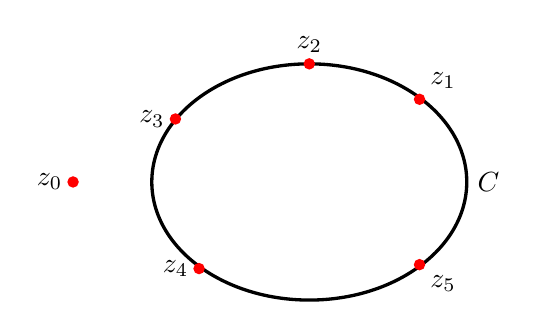
\begin{tikzpicture}[very thick]
  \draw (0,0) ellipse (2 and 1.5) (2,0) node [right] {$C$};
  \draw[red,fill] (-3, 0) circle (0.05) node [black, left] {$z_0$};
  \draw[red, fill] (1.4, 1.05) circle (0.05) node [black, above right] {$z_1$}
  (0,1.5) circle (0.05) node [black, above] {$z_2$}
  (-1.7,.8) circle (0.05) node [black, left] {$z_3$}
  (-1.4,-1.1) circle (0.05) node [black, left] {$z_4$}
  (1.4,-1.05) circle (0.05) node [black, below right] {$z_5$};
\end{tikzpicture}

%%% Local Variables:
%%% mode: latex
%%% TeX-master: "../main"
%%% End:

  \caption{In the first test family, we blow up the plane along $\{z_0, \dots, z_5\}$ as $z_0$ stays fixed and $z_1,\dots,z_5$ vary in a general 4-dimensional series on a fixed conic $C$.}
  \label{fig:FamilyB1}
\end{figure}

\begin{proposition}
  \label{prop:B1}
  Let $C$ be a plane conic, $Z \subset C$ a subscheme of length 5, and $z_0 \in \P^2$ a point not on $C$.
  Then the subscheme $Z \cup \{z_0\} \subset \P^2$ is admissible.
\end{proposition}
\begin{proof}
  The subscheme $Z' = Z \cup \{z_0\}$ is clearly curvilinear.
  Checking that $\mathcal I_{Z'} \otimes \O(3)$ is generated by its global sections is straightforward.
\end{proof}

We now formally define the family.
Let $H = \Hilb^5(C) \cong \P^5$ and let $B \cong \P^4 \subset H \cong \P^5$ be a general hyperplane.
Let $Z \subset B \times C$ be the restriction of the universal closed subscheme.
Set 
\[Z' = Z \sqcup B \times \{z_0\} \subset B \times \P^2.\]
Our family
\[\pi \colon X \to B\]
is the family of cubic surfaces associated to $Z' \subset B \times \P^2$ (see \autoref{def:cubicZ}).
It is easy to see that the family is good.
\begin{lemma}\label{prop:goodnessB1}
  The family $\pi \colon X \to B$ is good.
\end{lemma}
\begin{proof}
  We show that for every $b \in B$, the group $\Aut(X_b)$ is finite (see \autoref{ex:finaut}).
  By \autoref{prop:good}, it suffices to show that the group $\Aut(\P^2, Z_b')$ is finite.
  Since the support of $Z_b'$ is finite, it suffices to show that the subgroup of $\Aut(\P^2, Z'_b)$ that acts trivially on the support is finite.
  Let $\sigma \in \Aut(\P^2, Z'_b)$ act trivially on the support.
  Since $C$ is the unique conic containing $Z_b$, the element $\sigma$ must preserve $C$.
  Since $\sigma(z_0) = z_0$, and $\sigma$ preserves $C$, it must fix the pair of points $\Polar_C(z_0) \cap C$.
  Since $B \subset \Hilb^5C$ is general, we may assume that it does not contain the finitely many length 5 schemes supported on $\Polar_C(z_0) \cap C$.
  Then $\sigma$ fixes at least 3 points of $C$, namely the two points $\Polar_C(z_0) \cap C$ and the points of $Z \subset C$.
  It follows that $\sigma$ fixes all points of $C$ and hence all points of $\P^2$.
\end{proof}

Let us evaluate the degree 4 monomials in the Chern classes of the anti-canonical section bundle.
\begin{lemma}\label{lem:v1}
  Let $\mathcal V = \pi_* \left( \omega_{X/B}^{-1} \right)$.
  Then we have
  \[
    \int_{B_{1}}v_{1}^{4} = 16, \quad \int_{B_{1}}v_{1}^{2}v_{2} = 4,\quad \int_{B_{1}}v_{1}v_{3} =0,\quad \int_{B_{1}}v_2^{2} = 1,\quad \int_{B_{1}}v_{4} = 0.\]
\end{lemma}
\begin{proof}
By the construction of the cubic surface, we see that $\mathcal V$ is the rank 4 bundle
\[ \mathcal V = \pi_* (\mathcal I_{Z'} \otimes \omega_{\pi}^{-1}),\]
where $\pi \colon B \times \P^2 \to B$ is the first projection.
It contains the constant rank 2 bundle
\begin{equation}\label{eqn:v11}
  \pi_*\left( \mathcal I_{B \times C} \otimes \mathcal I_{B \times z_0} \otimes \omega_\pi^{-1} \right) = H^0\left(\mathcal I_{C} \otimes \mathcal I_{z_0} \otimes \omega_{\P^2}^{-1}\right) \otimes \O_{B},
\end{equation}
and the quotient is the rank 2 bundle $\pi_*\left( I_{Z/B \times C} \otimes \omega_\pi^{-1} \right)$.
To identify the quotient, note that $Z \subset B \times C$ is a divisor of class $(1,5)$ and $\omega^{-1}_{\pi}|_{B\times C}$ is isomophic to $\O(0,6)$.
Hence, $I_{Z/B \times C} \otimes \omega_\pi^{-1}$ is isomorphic to $\O(-1,1)$, and therefore
\begin{equation}\label{eqn:v12}
  \begin{split}
    \pi_*\left( I_{Z/B \times C} \otimes \omega_\pi^{-1} \right) \cong \O_{B}(-1)^{2}.
  \end{split}
\end{equation}
By combining \eqref{eqn:v11} and \eqref{eqn:v12}, we see that $\mathcal V$ is an extension
\begin{equation}\label{eqn:V1}
  0 \to \O_{B}^2 \to \mathcal V \to \O_{B}(-1)^2 \to 0.
\end{equation}
The Chern class calculation is now straightforward using the Whitney sum formula.
\end{proof}

Let us find the degree of the map to moduli $B \dashrightarrow \M$.
\begin{lemma}\label{lem:deg1}
  The degree of $B \dashrightarrow \M$ is $4320$.
\end{lemma}
\begin{proof}
  Consider space of marked cubic surfaces $\M^\dagger$, which is isomorphic to the configuration space of 6 ordered points on $\P^2$.
  We have the action of $S_5$ on $\M^\dagger$ via permutations of the last 5 points.
  The map $B \dashrightarrow \M$ lifts to
  \begin{equation}\label{eqn:b1lift}
    B \to \M^\dagger / S_5,
  \end{equation}
  where $b \in B$ is mapped to $(z_0, z_1 + \dots + z_5)|_b$.
  Let us compute the degree of this map.
  Given a general $(y_0, y_1 + \dots + y_5)$ in $\M^\dagger / S_5$, there is a unique conic $Q$ through $y_1 + \dots + y_5$.
  Note that there exists an automorphism of $\P^2$ that takes $(C, z_0)$ to $(Q, y_0)$, and such an automorphism is unique up to automorphisms preserving $(C, z_0)$.
  Suppose, under one such automorphism, $y_1 + \dots + y_5 \subset Q$ is taken to $z_1' + \dots + z_5' \subset C$.
  We must find out how many points of $B$ are equivalent to $z_1' + \dots + z_5'$ up to an automorphism of $\P^2$ preserving $(C, z_0)$.
  Let $w_0 + w_\infty \subset C$ be the scheme $\Polar_C(z_0) \cap C$.
  Then we have
   \[\Aut(\P^2, C, z_0) = \Aut(C, w_0 + w_{\infty}) \cong \G_m \times \Z/2\Z. \]
   Choose an isomorphism $C \cong \P^1$ such that $w_0$ and $w_\infty$ are identified with $[0:1]$ and $[1:0]$.
   Then the $\G_m$ corresponds to the diagonal $\G_m \subset \PGL_2$ and the $\Z/2\Z$ corresponds to the swapping of the two homogeneous coordinates.
   Write $z_1' + \dots + z_5'$ as the vanishing locus of a binary quintic form $F$.
   It is easy to see that under the action of the $\G_m$, the closure of the orbit of $V(F)$ in $\Hilb^5 C \cong \P^5$ is a rational normal curve.
   Hence, a general hyperplane $B$ intersects the orbit in 5 points.
   Accounting for the additional $\Z/2\Z$, we conclude that there are precisely 10 points of $B$ equivalent to $z_1' + \dots + z_5'$ up to an automorphism of $\P^2$ preserving $(C, z_0)$.
   Thus, the degree of the map in \eqref{eqn:b1lift} is 10.

   Since the degree of $\M^\dagger \to \M$ is $51840$, the degree of $B \to \M$ is
   \[51840/5! \times 10 = 4320.\]
\end{proof}

Using \autoref{prop:goodisgood} and the computation of the Chern classes and the degree, we obtain the following relation on the undetermined coefficients of $[\Orb(X)]$ in
\eqref{eqn:chernexpansion} for a general cubic surface $X$:
\begin{align}
  \label{eq:relation1}
  16 \cdot a_{1^4} + 4 \cdot a_{1^2 2} + a_{2^2} = 4320.
\end{align}

%------------------------------------------------------------------------------------

\subsection{The second test family}
\label{sec:family-b_2}
We begin with an informal description of the family.
Forget the notation introduced in \autoref{sec:family-b_1}.
We take a smooth conic $C \subset \P^2$ and 7 distinct marked points $s_0, s_1, \dots, s_5, s_\infty$ on $C$.
Let $t \in \P^2$ be the pole, with respect to $C$, of the line joining $s_0$ and $s_\infty$.
We blow up the six points $s_1,\dots, s_5, t$ to get a cubic surface (see \autoref{fig:FamilyB2}).
As the 7 points vary on $C$, we get a 4-parameter family of cubic surfaces.

\begin{figure}
    \centering
    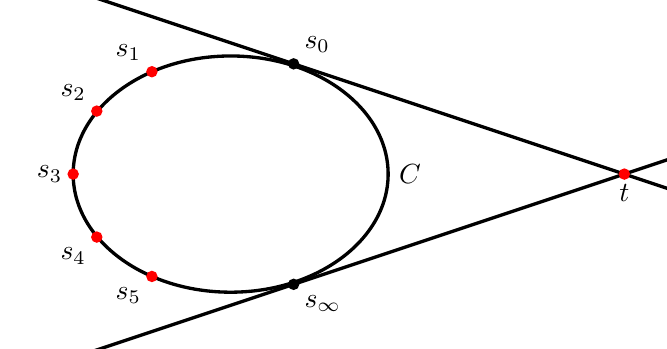
\begin{tikzpicture}[very thick]
  \draw (0,0) ellipse (2 and 1.5) (2,0) node [right] {$C$};
  \draw[shorten >=-3cm, shorten <=-3cm] (0.8, 1.4) -- (5,0);
  \draw[shorten >=-3cm, shorten <=-3cm] (0.8, -1.4) -- (5,0);

  \draw[red, fill] (5,0) circle (0.05) node [black, below] {$t$};
  \draw[fill] (0.8, 1.4) circle (0.05) node [above right] {$s_0$};
  \draw[fill] (0.8, -1.4) circle (0.05) node [below right] {$s_\infty$};

  \draw[red, fill]
  (-1, 1.3) circle (0.05) node [black, above left] {$s_1$}
  (-1.7, 0.8) circle (0.05) node [black, above left] {$s_2$}
  (-2, 0) circle (0.05) node [black, left] {$s_3$}
  (-1, -1.3) circle (0.05) node [black, below left] {$s_5$}
  (-1.7, -0.8) circle (0.05) node [black, below left] {$s_4$};
\end{tikzpicture}

%%% Local Variables:
%%% mode: latex
%%% TeX-master: "../main"
%%% End:

    \caption{
      In the second test family, we blow up the plane at the points $\{s_{1}, \dots, s_{5}, t\}$ as the seven points $\{s_1, \dots, s_5, s_0, s_\infty\}$ vary freely on a conic $C$.}
    \label{fig:FamilyB2}
  \end{figure}


We now make the construction more precise, and show how to use it construct a family of cubic surfaces over $\overline {\M}_{0,7}$.
Let $\phi \colon \mathcal C \to \overline \M_{0,7}$ be the universal curve with the universal sections denoted by $\sigma_0, \sigma_1, \dots, \sigma_5, \sigma_\infty$.
Let $\mathcal L$ be the line bundle $\sigma_\infty^*\left(\omega_\phi\right)$ on $\overline \M_{0,7}$.
As is customary, we denote its Chern class by $\psi_\infty$.
Consider the rank 2 vector bundle
\[ \mathcal A = \phi_* \O_{\mathcal C}\left(\sigma_\infty\right).\]
It is easy to check that the evaluation maps yield an isomorphism
\begin{align*}
  \mathcal A &\xrightarrow{\sim} \sigma_\infty^*\O_{\mathcal C}\left( \sigma_\infty \right) \oplus \sigma_0^*\O_{\mathcal C}\left( \sigma_\infty \right)\\
  &= \mathcal L^{-1} \oplus \O_{\overline \M_{0,7}}.
\end{align*}
Set $\overline {\mathcal C} = \P \mathcal A^\vee$ with the structure map $\overline \phi \colon \overline {\mathcal C} \to \overline \M_{0,7}$.
The evaluation map $\phi^*\mathcal A \to \O_{\mathcal C}\left(\sigma_\infty\right)$ yields a map $\gamma \colon \mathcal C \to \overline {\mathcal C}$.
The effect of $\gamma$ on a stable curve $(C, s_0, \dots, s_\infty)$ is to contract all irreducible components of $C$ not containing the marked point $s_\infty$.
The unique remaining $\P^1$ is identified with the corresponding fiber of $\overline \phi$.
Set $\overline \sigma_i = \sigma_i \circ \gamma$; these $\overline \sigma_i$ are sections of $\overline \phi \colon \overline {\mathcal C} \to \overline \M_{0,7}$.
They satisfy the following properties
\begin{itemize}
\item $\overline{\sigma}_{\infty}$ is disjoint from all the other sections, and
\item in each fiber of $\overline \phi$, the union of all seven sections
  is supported on at least three points.
\end{itemize}

We now invoke the relative 2-Veronese embedding
\[
\iota \colon \overline {\mathcal C} \to \mathcal P := \P \Sym^2 \mathcal A^\vee.
\]
Let $\rho \colon \mathcal P \to \overline{\M}_{0,7}$ be the structure morphism.
Then $\overline {\mathcal C} \subset \mathcal P$ is a family of smooth conics with 7 marked points $\sigma_0, \dots, \sigma_\infty$ satisfying the two properties above.

Let $\tau \colon \overline \M_{0,7} \to \mathcal P$ be the section obtained by fiberwise taking the pole with respect to $\overline {\mathcal C}$ of the line joining the points $\overline \sigma_0$ and $\overline \sigma_\infty$.
Here is an alternate description of $\tau$.
The direct sum decomposition $\mathcal A = \O \oplus \mathcal L^{-1}$ gives the decomposition
\[ \Sym^2 \mathcal A = \O \oplus \mathcal L^{-1} \oplus \mathcal L^{-2}.\]
In $\P \mathcal A^\vee$, the sections $\overline \sigma_0$ and $\overline \sigma_\infty$ correspond to the projections $\mathcal A \to \O$ and $\mathcal A \to \mathcal L^{-1}$, respectively.
Hence, in the Veronese embedding, they correspond to the projections $\Sym^2 A \to \O$ and $\Sym^2 A \to \mathcal L^{-2}$, respectively.
Using the quadratic form on $\Sym^2 \mathcal A$ given by the Veronese conic, it is easy to check that the section $\tau$ is given by the third projection $\Sym^2 A \to \mathcal L^{-1}$.

We let $\Sigma \subset \overline{\mathcal C}$ denote the closed subscheme associated to the divisor $\overline \sigma_1 + \dots + \overline \sigma_5$ and $\mathcal Z \subset \mathcal P$ the disjoint union $\Sigma \sqcup \tau$.
By \autoref{prop:B1}, $\mathcal Z \subset \mathcal P$ is a family of admissible subschemes.
We let
\[ \pi \colon \mathcal X \to \overline \M_{0,7}\]
be the family of cubic surfaces associated to $\mathcal Z \subset \mathcal P$ (see \autoref{def:cubicZ}).

\begin{lemma}  \label{prop:goodnessB2}
  The family $\pi \colon \mathcal X \to \overline \M_{0,7}$ is good.
\end{lemma}
\begin{proof}
  All fibers have finite automorphism groups by the same proof as \autoref{prop:goodnessB1}.
\end{proof}

We now compute the Chern classes of the anti-canonical section bundle.
\begin{proposition}\label{lem:v2}
  Let $\mathcal V = \pi_* \omega_{\pi}^{-1}$.
  Then we have
  \[
    \begin{split}
      \int_{\overline \M_{0,7}}v_{1}^{4} = 625&, \quad \int_{\overline \M_{0,7}}v_{1}^{2}v_{2} = 125,\quad \int_{\overline \M_{0,7}}v_{1}v_{3} = -25,\\
      &\int_{\overline \M_{0,7}}v_2^{2} = 25,\quad \int_{\overline \M_{0,7}}v_{4} = -6.
    \end{split}
  \]
\end{proposition}
For the proof, we use the following.
\begin{lemma}\label{lem:push}
  Let $\pi \colon P \to B$ be a $\P^1$-bundle with a section $\sigma$.
  Let $D \subset P$ be a divisor of relative degree $d$ with respect to $\pi$ with $d \geq -1$.
  Then, in the Grothendieck group of $B$, we have
  \[ [\pi_* \O(D)] = [\sigma^*\O(D)] + \dots + [\sigma^*\O(D-(d-1)\sigma)].\]
\end{lemma}
\begin{proof}
  We induct on $d$.
  Both sides are 0 for $d = -1$.
  The exact sequence
  \[ 0 \to \O(D-\sigma) \to \O(D) \to \O(D)|_\sigma \to 0\]
  pushed-forward to $B$ provides the induction step.
\end{proof}
\begin{proof}[Proof of \autoref{lem:v2}]
  Recall that $\mathcal X \to \overline \M_{0,7}$ is the cubic surface associated to $\mathcal Z \subset \mathcal P$ in the $\P^2$-bundle $\rho \colon \mathcal P \to \overline \M_{0,7}$.
  By construction, we have
  \[ \mathcal V = \rho_*(\mathcal I_{\mathcal Z} \otimes \omega^{-1}\rho).\]
  Hence, in the Grothendieck group of $\overline \M_{0,7}$, we have
  \begin{equation}\label{eqn:diff}
    [\mathcal V] = \rho_*(\omega_\rho^{-1}) - \rho_*(\omega_\rho^{-1}|_{\mathcal Z}).
  \end{equation}
  By the relative Euler sequence, we see that $\omega^{-1}_\rho$ is isomorphic to $\O_{\mathcal P}(3) \otimes \rho^* \det (\Sym^2 \mathcal A)^\vee$, and hence the first term in \eqref{eqn:diff} is
  \begin{equation}\label{eqn:diff1}
    \rho_*(\omega_\rho^{-1}) = \Sym^3(\Sym^2 \mathcal A) \otimes \mathcal L^3.
  \end{equation}
  Since $\mathcal Z$ is the disjoint union $\Sigma \cup \tau$, the second term is a sum
  \[ \rho_*(\omega_\rho^{-1}|_{\mathcal Z}) = \rho_*(\omega_\rho^{-1}|_{\tau}) + \rho_*(\omega_\rho^{-1}|_{\Sigma}). \]
  Since $\tau$ is defined by the surjection $\Sym^2 \mathcal A \to \mathcal L$, the restriction $\omega_\rho^{-1}|_\tau$ is trivial.
  To compute the restriction to $\Sigma$, we view $\Sigma$ as a divisor in $\overline{\mathcal C} = \P A^\vee$ and let $\lambda = \omega_\rho^{-1}|_{\overline C} = \O(6) \otimes \overline \phi^* \mathcal L^3$.
  Thus, in the Grothendieck group, we have
  \begin{equation}\label{eqn:diff2}
    \rho_*(\omega_\rho^{-1}|_{\Sigma}) = \overline\phi_*\left(\lambda\right) - \overline\phi_* \left( \lambda(-\Sigma)\right).
  \end{equation}
  We now use \autoref{lem:push} with the section $\sigma_\infty$ to compute the terms on the right hand side of \eqref{eqn:diff2}.
  Putting this together with \eqref{eqn:diff} and \eqref{eqn:diff1}, we get
  \[ [\mathcal V] = \mathcal L^{-3}+ \mathcal L^{1}+ \mathcal L^{-1}+ \mathcal L^{-2}\]
  in the Grothendieck group.
  The result now a simple computation using $c_1(\mathcal L) = \psi_\infty$ and $\int_{\overline \M_{0,7}} \psi_\infty^4 = 1$.
\end{proof}

Having computed the Chern classes, we need to find the degree of the map $\overline \M_{0,7} \dashrightarrow \M$.
\begin{proposition}
  The degree of $\overline \M_{0,7} \dashrightarrow \M$ is $103680$.
\end{proposition}
\begin{proof}
  The map lifts to $\overline \M_{0,7} \dashrightarrow \M^\dagger$.
  Since the degree of $\M^\dagger \to \M$ is $51840$, we must prove that the degree of $\overline \M_{0,7} \dashrightarrow \M^\dagger$ is $2$.

  Recall that $\M^\dagger$ is isomorphic to the configuration space of 6 points in $\P^2$.
  Given a general 6-tuple of points $(s_1,\dots, s_5, y)$ in $\P^2$, there is a unique conic $C$ passing through $s_1,\dots, s_5$.
  Let $x$ and $y$ be the two points of $\Polar(t) \cap C$.
  Then the two pre-images of $(s_1,\dots, s_5, t)$ in $\overline \M_{0,7}$ are $(C, x, s_1, \dots, s_5, y)$ and $(C,y, s_1, \dots, s_5, x)$.
  The proof is thus complete.
\end{proof}

Using \autoref{prop:goodisgood} and the computation of the Chern classes and the degree, we obtain the following relation on the undetermined coefficients of $[\Orb(X)]$ in
\eqref{eqn:chernexpansion} for a general cubic surface $X$:
\begin{align}
  \label{eq:relation2}
  625 a_{1^{4}} + 125 a_{1^{2}2} - 25a_{13} + 25a_{2^2} - 6 a_{4} = 103680.
\end{align}

%------------------------------------------------------------------------------


\subsection{Family $B_3$}
\label{sec:family-b_3}


\begin{figure}[!]
    \centering
    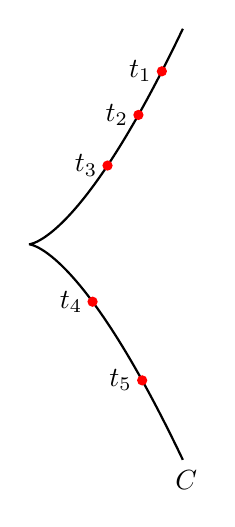
\begin{tikzpicture}[thick]
  \draw [domain=0:1.4, samples=100] 
  plot ({\x^2}, {\x^3} )
  plot ({\x^2}, {-\x^3} );
  \draw (2, -3) node {$C$};
  \draw[red, fill] (1.3^2, 1.3^3) circle (0.05) node [black, left] {$t_1$};
  \draw[red, fill] (1.18^2, 1.18^3) circle (0.05) node [black, left] {$t_2$};
  \draw[red, fill] (1.0^2, 1.0^3) circle (0.05) node [black, left] {$t_3$};
  \draw[red, fill] (1.2^2, -1.2^3) circle (0.05) node [black, left] {$t_5$};
  \draw[red, fill] (0.9^2, -0.9^3) circle (0.05) node [black, left] {$t_4$};
\end{tikzpicture}

%%% Local Variables:
%%% mode: latex
%%% TeX-master: "../main"
%%% End:

    \caption{In the family $B_3$, we blow up the points $t_i$ for $i = 1, \dots, 5$ and a fixed point $t_\infty$ at infinity (not shown) as the points $\{t_1, \dots, t_5\}$ move freely on a fixed cuspidal cubic $C$ with a flex at $t_\infty$.}
    \label{fig:FigureB3}
\end{figure}


Let us reset notation once again.  Our third family is a variant of
the family in the previous section \autoref{sec:family-b_2}.  It is
parametrized by the base variety
$$B_{3} := \hM_{0,7}.$$

Here, $\hM_{0,7}$ is a particular Hassett space parametrizing
${\bf w}$-stable $7$-pointed genus $0$ curves, where
$${\bf w} = \left(1-\epsilon, \epsilon, \dots, \epsilon, 1-3 \epsilon \right), 0 < \epsilon \ll 1$$
is the weight vector on the marked points
$(s_{0}, s_{1}, \dots, s_{5}, s_{\infty})$ on a genus $0$ curve.

Before getting buried in details, we explain the basic construction of
the family of cubic surfaces over the interior, $\M_{0,7}$.  Begin
with $(C, s_{0}, s_{1}, \dots, s_{5}, s_{\infty})$, a smooth rational
curve with $7$ distinct marked points, and choose a map
$$\nu: C \to \P^{2},$$ birational onto its image
$\nu(C)$, which is a {\sl cuspidal cubic curve with cusp point
  $\nu(s_{0})$ and unique flex point $\nu(s_{\infty})$.}  Let
$Z = \nu(\{s_{1}, \dots, s_{5}, s_{\infty}\}) $, and now assign the
cubic surface $\Bl_{Z}\P^{2}$.  The main objective of this section is
to demonstrate that this assignment extends over the boundary of
$\hM_{0,7}$, yielding a good family of cubic surfaces from which we
can extract one more relation.

Before starting the analysis, we make some remarks: The need for using
the alternate compactification $\hM_{0,7}$ ultimately traces to the
requirement that our family must be good.  There are several possible
variants of the construction, but the reader will eventually realize
that, very often, there will be a few non-good fibers present.


We assume the reader is familiar with the intersection theory of
$\o{\M}_{0,n}$.  Therefore, we will at times translate intersection
products on $\hM_{0,7}$ into calculations on $\o{\M}_{0,7}$, and then
leave it to the reader to check the results there.

\subsubsection{The spaces $\hM_{0,n}$}
\label{sec:spaces-hm_0-n}

In order to carry out the calculations needed for our third relation,
we need to investigate the basic geometry of a series of
Hassett-spaces which we denote by $\hM_{0,n}$.  We do that in this
section.

\begin{definition}
  \label{def:hM0n} For each $n \geq 4$, we define $\hM_{0,n}$ to be
  the compactification of $\M_{0,n}$ by ${\bf w}$-stable, $n$-pointed,
  genus $0$ curves, where
  $${\bf w} = \left(1- \epsilon, \epsilon, \dots, \epsilon, 1-(n-4)\epsilon \right), 0 < \epsilon \ll 1.$$
\end{definition}

We will denote a ${\bf w}$-stable curve by
$(C, s_{0}, s_{1}, \dots, s_{n-2}, s_{\infty})$.  The indices are
meant to indicate that the two points $s_{0}$ and $s_{\infty}$ are two
``more interesting'' points, as will become apparent in the next
paragraph.

The pointed curves $(C, s_{0}, s_{1}, \dots, s_{n-2}, s_{\infty})$
parametrized by $\hM_{0,n}$ are actually very simple to describe:

\begin{itemize}
\item $C$ is a {\sl smooth} rational curve,
\item $s_{0}$ and $s_{\infty}$ must be distinct,
\item at most one of the $s_{i}$, $i=1, \dots, n-2$ can coincide with
  $s_{0}$,
\item at most $n-4$ of the $s_{i}$, $i=1, \dots, n-2$ can coincide
  with $s_{\infty}$.
\item there are no constraints on how the points $s_{i}$,
  $i=1, \dots, n-2$ can coincide with each other.
\end{itemize}
Therefore, the universal curve $$\varphi: \cC \to \hM_{0,n}$$ is in
fact a $\P^{1}$-bundle, the projectivization of a particular rank $2$
vector bundle $\mathcal{W}$ on $\hM_{0,n}$. We let
$\sigma_{i} \subset \cC$,
$i \in \left\{0,1,2, \dots, n-2, \infty\right\}$ denote the universal
sections providing the marked points, and we denote by
\begin{align}
  \label{eq:stab}
  \zeta: \overline{\M}_{0,n} \to \hM_{0,n}
\end{align}
the stabilization morphism.  We will sometimes use $\zeta$ to
pull-back enumerative calculations on $\hM_{0,n}$ back to
$\overline{\M}_{0,n}$, where they are better understood.

\paragraph{Divisor classes on $\hM_{0,n}$}
\label{sec:divisor-classes-hm_0}

Certain divisors on $\hM_{0,n}$  play an essential role in our
computations, so we take this section to introduce them.

\begin{definition}
  \label{def:psihats} We let $\hL_{0}, \hL_{\infty}$ denote the line
  bundles
  $\omega_{\varphi}|_{\sigma_{0}},
  \omega_{\varphi}|_{\sigma_{\infty}}$, respectively, and let
  $\hpsi_{0}, \hpsi_{\infty} \in A^{1}(\hM_{0,n})$ denote their first
  Chern classes.
\end{definition}

Since the sections $\sigma_{0}$ and $\sigma_{\infty}$ are disjoint, it
follows that
\begin{align}
  \label{eq:opposites}
  \hpsi_{0} + \hpsi_{\infty} = 0.
\end{align}


Finally, we indicate the simple relationship between $\hpsi_{0}$ on
$\hM_{0,n}$ with $\psi_{0}$ on $\o{\M}_{0,n}$.  Let
$\delta_{\{i,0\}}, i=1, \dots, n-2$ denote the boundary divisor in
$\o{\M}_{0,n}$ whose general point corresponds to the union of two
marked $\P^{1}$'s, one of which contains only $0$-th and $i$-th marked
points.



Then,
\begin{align}
  \label{eq:relationpsis}
\zeta^{*}(\hpsi_{0}) = \psi_{0} - \sum_{i \in \{1, \dots, n-2\}} \delta_{\{i,0\}}.  
\end{align}













\begin{definition}
  \label{def:boundary}
  For each distinct pair of indices
  $i,j \in \{0, 1, 2, \dots, n-2, \infty \}$, we define
  $\Delta_{i,j} \subset \hM_{0,n}$ to be the divisor over which the
  sections $\sigma_{i}$ and $\sigma_{j}$ intersect, and we set
  $$\Delta_{\infty} = \sum_{i \in \{1, \dots, n-2 \}}
  \Delta_{i,\infty}.$$
\end{definition}

The specific boundary divisors $\Delta_{i, \infty}$, where the section
$\sigma_{i}$ collides with $\sigma_{\infty}$ will play an especially
important role in our calculations will be important for us, so we
briefly collect some observations about them:
\begin{itemize}\label{item:boundaryprops}
\item Each boundary divisor $\Delta_{i,\infty} \subset \hM_{0,n}$ is
  naturally isomorphic to $\hM_{0,n-1}$ via a map
  $$\eta_{i}: \hM_{0,n-1} \to \hM_{0,n}$$ that sends
  $(C, s_{0}, \dots, s_{n-3}, s_{\infty})$ to
  $(C, s_{0}, \dots, s_{i-1}, s_{i}=s_{\infty}, s_{i+1} \dots,
  s_{\infty})$.

  In the same way, if $i \neq j$, then the intersection
  $\Delta_{i,\infty} \cap \Delta_{j, \infty}$ is isomorphic to
  $\hM_{0,n-2}$ via a similarly defined map
  $$\eta_{i,j}: \hM_{0,n-2} \to \hM_{0,n},$$ and so on.  This provides a
  nice inductive structure among the Hassett spaces $\hM_{0,n}$.
  
\item Under $\eta$, we clearly have $\eta^{*}\hpsi_{0} = \hpsi_{0}$
  and $\eta^{*}\hpsi_{\infty} = \hpsi_{\infty}.$
\item We have:
\begin{align}\label{eq:pullbackdelta}
  \eta^{*}([\Delta_{i,\infty}]) = -\hpsi_{\infty} \in A^{1}(\hM_{0,n-1}).
\end{align}
To see this, first note that
$\Delta_{i, \infty} = \varphi_{*}(\sigma_{i}\sigma_{\infty})$, and so
$\eta^{*}([\Delta_{i,\infty}]) = \varphi_{*}(\sigma_{\infty}^{2})$,
where the latter equation is happening in the divisor class group of
$\hM_{0,n-1}$.  But
$\varphi_{*}(\sigma_{\infty}^{2}) = - \hpsi_{\infty}$, and the claim
follows.
\end{itemize}


\paragraph{Computing integrals in $\hM_{0,n}$}

These observations are enough to compute, using an inductive method,
any top degree integral involving $\hpsi_{0}, \hpsi_{\infty},$ and the
boundary divisors $\Delta_{i, \infty}$.

\begin{example}
  \label{ex:toppsi}
  Let's first indicate how to
  compute $$\int_{\hM_{0,n}}\hpsi_{0}^{n-3}.$$ Using
  \eqref{eq:relationpsis}, this amounts to computing
  $$\int_{\o{\M}_{0,n}} \left(\psi_{0} - \sum_{i \in \{1, \dots, n-2\}} \delta_{\{i,0\}}\right)^{n-3}.$$
  Now, in the Chow ring of $\o{\M}_{0,n}$, recall that:
  \begin{itemize}
  \item $\psi_{0} \cdot \delta_{\{i,0\}} = 0$, 
  \item $\delta_{\{i,0\}} \cdot \delta_{\{j,0\}} = 0$ for $i \neq j$,
    and
  \item $\int_{\o{\M}_{0,n}}\delta_{\{i,0\}}^{n-3} = (-1)^{n}$, for
    all $i$, and
  \item $\int_{\o{\M}_{0,n}} \psi_{0}^{n-3} = 1$.
  \end{itemize}

  Using these, we deduce:
  \begin{align}
    \label{eq:hpsitop}
    \int_{\hM_{0,n}}\hpsi_{0}^{n-3} = -(n-3). 
  \end{align}
\end{example}

Next, we do an example involving $\Delta_{i, \infty}$'s.

\begin{example}
  Consider
  $$\int_{\hM_{0,7}} \Delta_{i, \infty}^{2}\Delta_{j, \infty}^{2},$$
  where $i \neq j$.  Using the parametrization
  $\eta_{i,j} : \hM_{0,5} \to \Delta_{i,\infty} \cap
  \Delta_{j,\infty}$, we see that this integral is the same as
  $$\int_{\hM_{0,5}}\eta_{i,j}^{*}[\Delta_{i, \infty}] \cdot \eta_{i,j}^{*}[\Delta_{j, \infty}],$$
  which in turn is equal to
  $$\int_{\hM_{0,5}}(-\hpsi_{\infty})^{2} = \int_{\hM_{0,5}}\hpsi_{0}^{2} = -2,$$
  as seen by combining \eqref{eq:hpsitop} with previous observations
  on how boundary divisors pull back along $\eta_{i}$ maps.
\end{example}

The intersection theory described in this subsection yields:

\begin{lemma}
  \label{lemma:monomials} On $\hM_{0,7}$ we have:
  \begin{align}
    \int_{\hM_{0,7}}\widehat{\psi}_{0}^{4}& = -4, \\ \nonumber
    \int_{\hM_{0,7}}\widehat{\psi}_{0}^{3}\Delta_{\infty}& = -15, \\ \nonumber
    \int_{\hM_{0,7}}\widehat{\psi}_{0}^{2}\Delta_{\infty}^{2}& = -55, \\ \nonumber
    \int_{\hM_{0,7}}\widehat{\psi}_{0}\Delta_{\infty}^{3}& = -195, \\ \nonumber
    \int_{\hM_{0,7}}\Delta_{\infty}^{4}& = -655
  \end{align}
\end{lemma}

\subsubsection{Construction of the family $\cX/\hM_{0,7}$}
\label{sec:constr-family-hM07}

Let us proceed to the formal construction of our family, starting with
the universal curve
$$\varphi: \cC \to \hM_{0,7}.$$
The idea is to map $\cC$ to a relative cuspidal cubic curve in a
$\P^{2}$-bundle so that $\sigma_{0}$ becomes the cusp point and
$\sigma_{\infty}$ becomes the flex point.


Consider the rank $2$
vector bundle $\mathcal{A} = \varphi_{*}\O_{\cC}(\sigma_{\infty})$ --
since $\sigma_{\infty}$ and $\sigma_{0}$ are disjoint, and since
$\O_{\cC}(\sigma_{\infty})|_{\sigma_{\infty}} = \hL_{\infty}^{-1}$ and
$\O_{\cC}(\sigma_{0})|_{\sigma_{0}} \simeq \O_{\hM_{0,7}}$, it follows
that
$$\mathcal{A} \simeq \O_{\hM_{0,7}} \oplus \hL_{\infty}^{-1}.$$
We emphasize that the above direct sum decomposition is induced by
applying $\varphi_{*}$ to the restriction map
$\O_{\cC}(\sigma_{\infty}) \to \O_{\cC}(\sigma_{\infty})|_{\sigma_{0}
  \cup \sigma_{\infty}}.$

  Next, consider the subbundle
  \begin{align}
    \label{eq:S}
    \mathcal{S} = :\O_{\hM_{0,7}} \oplus \hL_{\infty}^{-2} \oplus \hL_{\infty}^{-3} \subset \Sym^{3} \mathcal{A} = \O_{\hM_{0,7}} \oplus \hL_{\infty}^{-1} \oplus \hL_{\infty}^{-2} \oplus \hL_{\infty}^{-3},
  \end{align}
  and denote by
  \begin{align}
    \label{eq:nu}
    \nu: \cC \to \P \mathcal{S}^{\smvee}
  \end{align}
  the $\hM_{0,7}$-morphism induced by the surjection
  $\varphi^{*}\mathcal{S} \to \O_{\cC}(3\sigma_{\infty})$. Denote by
  $\rho: \P \mathcal{S}^{\smvee} \to \hM_{0,7}$ the $\P^{2}$-bundle
  structural map.  Fiber-by-fiber, the effect of $\nu$ is to map the
  fibers of $\cC$ to a cuspidal cubic curve, with $\nu(\sigma_{0})$
  the cusp point and $\nu(\sigma_{\infty})$ the flex point.

  We denote by $\mathcal{Z} \subset \cC$ the union of the six sections
  $\sigma_{1}, \dots, \sigma_{\infty}$.  Because at most one of the
  sections $\sigma_{i}, i \in \{1, \dots, \infty\}$ is allowed to
  intersect $\sigma_{0}$ (which becomes the cusp under $\nu$), it
  follows that $\nu|_{\mathcal{Z}}:\mathcal{Z} \to \nu(\mathcal{Z})$
  is an isomorphism. As will be demonstrated in
  \autoref{sec:goodness3}, every member of the family of length $6$
  subschemes $\nu(\mathcal{Z}) \subset \P \mathcal{S}^{\smvee}$ is
  admissible, and has a {\sl good} associated cubic surface.
  Therefore, our attention is brought upon the natural rank $4$ bundle
  \begin{align}
    \label{eq:V3}
    \V := \rho_{*}\left(\omega_{\rho}^{-1} \otimes \mathcal{I}_{\nu(\mathcal{Z})}\right)
  \end{align}
  of our claimed good family $$\pi: \cX \to \hM_{0,7},$$ with
  $\cX := \Bl_{\nu(\mathcal{Z})}\P \mathcal{S}^{\smvee}$.


\subsubsection{Goodness}
\label{sec:goodness3}

Here we address the goodness of the family
$\pi: \mathcal{X} \to B_{3}$. We let $$T \subset B_{3} = \hM_{0,7}$$
denote the finite set parametrizing marked curves
$(C, s_{0}, s_{1}, \dots, s_{5}, s_{\infty})$ where three of the
$s_{i}, i=1, \dots, 5$ coincide with $s_{\infty}$.  $T$ consists of
${5 \choose 3 } = 10$ points.  Using \autoref{prop:good}, it will be
relatively easy to show that $\pi: \mathcal{X} \to B_{4}$ is good over
the open set $B_{3} \setminus T$.  The argument showing that the
fibers over $T$ are also good is quite a bit more involved.  In the
interest of exposition, we have placed it in \autoref{sec:goodnessA5}.




\autoref{theorem:goodcusp} below essentially states that
$\pi : \mathcal{X} \to B_{3}$ is a good family over the open set
$B_{3} \setminus T$. The following elementary lemma, which we leave to
the reader, contains simple observations about automorphisms of
$\P^{2}$.

\begin{lemma}
  \label{lemma:identity} Suppose $g \in \Aut(\P^{2})$ satisfies one of:
  \begin{enumerate}
  \item $g$ restricts to the identity on a line $L \subset \P^{2}$ and
    also fixes two points outside $L$, or
  \item $g$ restricts to the identity on a line $L$, preserves another
    line $L'$ and fixes a point outside $L \cup L'$, or
  \item $g$ fixes $4$ points, no three collinear.
  \end{enumerate}
  Then $g = \id$.
\end{lemma}

\begin{proof}
  Omitted.
\end{proof}

\begin{theorem}
  \label{theorem:goodcusp}
  Let $C \subset \P^{2}$ be a cuspidal cubic, and let
  $s_{i} \in C, i \in \{1, \dots, 5, \infty \}$ be six, not
  necessarily distinct, points satisfying:
  \begin{enumerate}
  \item At most one $s_{i}$ is the cusp point,
  \item $s_{\infty}$ is the flex point of $C$, and
  \item at most {\bf two} $s_{i}, 1 \leq i \leq 5$ are equal to $s_{\infty}$.
  \end{enumerate}
  
  The length $6$ subscheme $Z := s_{1} + \dots + s_{5} + s_{\infty}$,
  interpreted as a divisor on $C$, is admissible and the associated
  cubic $X_{Z}$ is good.
\end{theorem}

\begin{proof}
  First note that since no length $4$ subscheme of $Z$ is contained in
  a line, it follows that the length $5$ subscheme
  $Z' := s_1 + s_2 + s_3 +s_4 +s_5$ is contained in a unique conic,
  which we denote by $Q$.

  The verification proceeds in cases, depending on the rank of the
  conic $Q$ and its relative position with respect to the cuspidal
  cubic $C$.  Observe first that every element in the identity
  component of $\Aut(\P^{2},Z)$ must preserve the conic $Q$. So, in
  light of \autoref{prop:good} it suffices to show that there are only
  finitely many elements in $\Aut(\P^{2},Z)$ preserving $Q$.  Let
  $g \in \Aut(\P^{2},Z)$ denote an arbitrary element in the identity
  component---we must deduce in every case that $g = \id$.  This
  strategy works in the first four cases. The fifth case proceeds
  differently, and appeals to the classification of semi-stable cubic
  surfaces.

  
  {\bf Case 1}: {\sl $Q$ is smooth and $s_{\infty} \notin Q$.}    Then
  $g$ must preserve the pair of points $\Polar(s_{\infty})$. Since $Z$
  is a subscheme of the irreducible cubic curve $C$, it follows that
  $Z'$ must have multiplicity at most $2$ at each of the pair of
  points $\Polar(s_{\infty})$.  This implies that $Z' \subset Q$ is
  supported on at least three points, and so $g$ is an automorphism of
  $Q$ fixing three points, i.e. $g = \id$.

  

  {\bf Case 2}: {\sl $Q$ is smooth and $s_{\infty} \in Q$.}  Let
  $C^{\circ}$ denote the smooth part of $C$. The classical chord and
  tangent method makes $C^{\circ}$ isomorphic to the additive group
  $\G_{a}$, with origin corresponding to $s_{\infty}$. If
  $Z \subset Q$ were supported on less than three points, necessarily
  $s_{\infty}$ and, say $s_{1}$, then, given condition (3) we deduce
  that $s_{1}$ must be contained in $C^{\circ}$ and must be a torsion
  point in the group law, meaning $s_{1} = s_{\infty}$. Thus, $Z$
  would have to be entirely supported on $s_{\infty}$, which is
  contrary to assumption.  Since $Z$ has at least three points of
  support, we deduce $g =\id$.

  
  {\bf Case 3}: {\sl $Q$ is twice a line $L$.} $L$ cannot be the flex
  line at $s_{\infty}$, because it would force $Z$ to be
  $6 s_{\infty}$, violating condition (3).  Nor can $L$ be the unique
  line joining $s_{\infty}$ and the cusp of $C$, since then the
  support of $Z$ would have to contain that cusp with multiplicity at
  least $2$, contrary to condition (1). Thus, $L$ meets $C$
  transversely at three distinct smooth points, including
  $s_{\infty}$.  Without loss of generality, we may assume
  $Z = 2s_1 + 2s_2 + 2s_{\infty}$, where
  $L \cap C = s_{1}+s_{2} + s_{\infty}$.

  
  Now, $g \in \Aut(\P^{2},Z)$ fixes three points on $L$, and hence
  restricts to the identity on $L$. Let
  $q_{1,2}, q_{1, \infty}, q_{2,\infty}$ denote the corresponding
  pairwise intersections of the three tangent lines to $C$ at
  $s_1, s_2, s_{\infty}$. $q_{1,2}, q_{1, \infty},$ and
  $ q_{2,\infty}$ are distinct: If two coincided at a point $p$, then
  $p$ must be a point on the flex line, and must therefore not lie on
  $C$. Projecting $C$ from $p$ would yield an order $2$ ramification
  point at $s_{\infty}$, two simple ramification points at 
  $s_{1}, s_{2}$ and another ramification point at the cusp.  This
  exceeds the length $4$ ramification scheme given by the
  Riemann-Hurwitz formula for a degree $3$ map between rational
  curves.  Thus, $g$ fixes $L$, and fixes at least two other points
  outside $L$; by \autoref{lemma:identity}, $g =\id$.

  
  {\bf Case 4}: {\sl $Q$ is the union of two distinct lines
    $L \cup M$, neither of which is the flex line at $s_{\infty}$.}
  Let $x$ denote the point $L \cap M$, and {\sl first assume that
    $x \notin C$.} $Z'$ must contain at least two points on each of
  the lines. Since $g$ must fix $x$, we can apply
  \autoref{lemma:identity} to deduce $g =\id$ in this case.

  Next, assume $x \in C$: $x$ is not the cusp point, because then
  there is no room for $Z'$, given condition (1). We leave it to the
  reader to check all combinatorial possibilities in this situation,
  depending on whether $L$ and $M$ are tangent to $C$ or not.  All
  situations here are accounted for by \autoref{lemma:identity}.

  {\bf Case 5}: {\sl $Q$ is the union of two distinct lines
    $L \cup M$, where $M$ is the flex line through $s_{\infty}$.} This
  is the most interesting case.  Once again, let $x = L\cap M$.  If
  $x \in C$, $x$ must be the flex point $s_{\infty}$, and $Z$ would
  have to have multiplicity at least $4$ at $s_{\infty}$, violating
  condition (3).

  So, we can assume $x \notin C$.  There is now only one option for
  $Z$: $Z$ must equal $Q \cap C$.  In this case, $\Aut(\P^{2}, Z)$ has
  positive dimensional automorphism group, and therefore
  \autoref{prop:good} does not apply.  Instead, the reader can check
  that $X_{Z}$ is a normal cubic surface with only $A_{1}$ and $A_{2}$
  singularities.  Hence $X_{Z}$ is GIT semi-stable.  Semi-stable
  surfaces are automatically good, finishing this case.
  
\end{proof}

  
It remains to prove that the finitely many fibers of
$\pi: \mathcal{X} \to B_{3}$ over $T \subset B_{3}$ are good.  Since
this argument is rather involved (and contains a method of independent
interest), we have moved it to \autoref{sec:goodnessA5}.

\begin{corollary}
  \label{cor:good3} $\pi: \cX \to B_{3}$ is good.
\end{corollary}

\subsubsection{The bundle $\V$ and its Chern classes}
\label{sec:bundle-v3}

As usual, we must compute the Chern classes of
$\V = \pi_{*}\left( \omega_{\pi}^{-1} \right)$.  The analysis runs
parallel to that found in \autoref{sec:chern-classes-v2}, and so we
skip the details, and report the results:

\begin{proposition}
  \label{prop:chernV3} The total Chern polynomial of $\V$ is:
  \begin{align}
    \label{eq:chernV3}
    c(\V) = \frac{1+\hpsi_{0}t}{1-4 \hpsi_{0}t}\left(1-\Delta_{\infty}t \right) \left(1 + (\hpsi_{0}-\Delta_{\infty})t \right)  \left(1 + (2\hpsi_{0}-\Delta_{\infty})t \right) \left(1 + (3\hpsi_{0}-\Delta_{\infty})t \right).
  \end{align}

  Furthermore, we have:
  \begin{align}
    \label{eq:monomialsV3}
    \int_{B_{3}}v_{1}^{4}& = 3436, \\ \nonumber
    \int_{B_{3}} v_{1}^{2}v_{2}& = 1076,\\ \nonumber
    \int_{B_{3}} v_{2}^{2}& = 316, \\ \nonumber
    \int_{B_{3}} v_{1}v_{3}& = 116, \\ \nonumber
    \int_{B_{3}} v_{4}& = 0. \nonumber
  \end{align}
\end{proposition}

\begin{proof}
  Mimic the analysis done in \autoref{sec:chern-classes-v2} to
  identify $c(V)$, and use the calculations in
  \autoref{lemma:monomials} to compute the monomials.
\end{proof}

\subsubsection{Third relation}
\label{sec:third-relation}

The degree of the natural map
$\mu': B_{3} \dashrightarrow \M^{\dagger}$ is $20$, by
\autoref{theorem:Schubert}. Therefore, by compiling all that we have
calculated in this section, we finally obtain our third relation:
\begin{align}
  \label{eq:relation3}
  3436a_{1^4} + 1076a_{1^{2}2} + 116 a_{13} + 316 a_{2^{2}} = 20 \times 51840.
\end{align}




%----------------------------------------------------------------------------



\subsection{Family $B_4$}




\label{sec:family-b_4}

We construct our fourth family $\pi: \cX \to B_4$ by starting with a
quintic del Pezzo surface $S$ (the blow up of the plane at four
general points) and, informally, ``blowing up $S$ at two points which
vary freely.''  The complication arises because we get a non-good
cubic surface by blowing up the surface $S$ at a pair of points
contained in one of its ten lines.  Most effort is concentrated on
resolving this issue.

The surface $S$ has $10$ exceptional lines which we denote by
$L_{1}, \dots, L_{10}$.  Each line $L_{i}$ meets exactly three other
(mutually disjoint) lines, and we let $T_{i} \subset S$ denote their
union. Furthermore, we let $\tau_{i} \subset L_{i}$ denote
$T_{i} \cap L_{i}$.

We let $S^{[2]}$ denote the Hilbert scheme of
pairs of points on $S$.  $S^{[2]}$ contains $10$ disjoint $\P^{2}$'s,
$\Lambda_1, \dots, \Lambda_{10}$, namely the Hilbert schemes
$L_{i}^{[2]}$ parametrizing degree $2$ subschemes contained in the
lines $L_{i}$. Let $\Lambda = \cup_{i}\Lambda_{i}$.  The crux of this
section is to show that the blow up $\Bl_{\Lambda}S^{[2]}$ hosts a
good family of cubic surfaces.


We let $\pi_{1}, \pi_{2}$ denote the projections of $S^{[2]} \times S$
to either factor, and denote by
$$\mathcal{Z} \subset S^{[2]} \times S$$ the universal subscheme. 

\subsubsection{Construction of $B_4$}
\label{sec:construction-b_4}





First, it is easy to see (we leave the verification to the reader)
that the open set
\begin{align} 
  \label{eq:UB3}
  U := S^{[2]} \setminus \Lambda
\end{align}
supports a good family of cubic surfaces, namely
\begin{align}
  \label{eq:XUB3}
  \cX^{\circ} := \Bl_{\mathcal{Z}_{U}}(U \times S).
\end{align}


However, when we extend $\cX^{\circ}$ in the naive way over $S^{[2]}$
the family acquires non-good fibers, namely unions of quadrics and
planes, and therefore we must modify $S^{[2]}$ along $\Lambda$.

Let
\begin{align}
  \label{eq:S2tilde}
  \widetilde{S^{[2]}} := \Bl_{\Lambda}S^{[2]}
\end{align}
denote the blow-up with blow-down map
$\beta: \widetilde{S^{[2]}} \to S^{[2]}$.  Let
$E_{i} = \beta^{-1}(\Lambda_{i})$, $i=1, \dots, 10$ denote the
components of the of the exceptional divisor of the blow-up; $\beta$
expresses $E_{i}$ as a $\P^{1}$-bundle over $\Lambda_{i}$.

Next, let $\widetilde{Z} := \widetilde{S^{[2]}} \times_{S^{[2]}} Z$
denote the fiber-product; $\widetilde{Z}$ is a closed subscheme of the
product $\widetilde{S^{[2]}} \times S$, and is a finite, flat, degree
two cover of $\widetilde{S^{[2]}}$ under the first projection
$\tilde{\pi}_{1} : \widetilde{Z} \to \widetilde{S^{[2]}}.$

Inside the product $\widetilde{S^{[2]}} \times S$ we define the
smooth, closed, codimension $2$ subschemes
\begin{align}
  \label{eq:Fi}
  F_{i} := E_{i} \times L_{i};
\end{align}
we let $F := \cup_{i}F_{i}$.  We perform one more blow-up along $F$ to
get
\begin{align}
  \label{eq:Xtilde}
  \mathcal{Y} := \Bl_{F}\left( \widetilde{S^{[2]}} \times S \right),
\end{align}
and denote by $\eta: \mathcal{Y} \to \widetilde{S^{[2]}} \times S $
the blowdown.  The next lemma is critical to our construction.

\begin{lemma}
  The closed immersion
  $i: \widetilde{\mathcal{Z}} \hookrightarrow \widetilde{S^{[2]}}
  \times S$ lifts to a closed immersion
  $j: \widetilde{\mathcal{Z}} \hookrightarrow  \mathcal{Y}$.
\end{lemma}

\begin{proof}
  The main observation is that we have an equality of schemes
  \begin{align}
    \label{eq:Cartier}
    F_i \cap \widetilde{\mathcal{Z}} = \widetilde{\pi}_{1}^{-1}(E_i) \cap \widetilde{\mathcal{Z}}
  \end{align}
  for all $i=1, \dots, 10$, {\sl and therefore
    $F \cap \widetilde{\mathcal{Z}}$ is a Cartier divisor on
    $\widetilde{\mathcal{Z}}$}.  Thus, the natural blowdown map

  \begin{align}
    \label{eq:blowdown}
    \Bl_{F \cap \td{\mathcal{Z}}}\td{\mathcal{Z}} \to \td{\mathcal{Z}}
  \end{align}
  is an isomorphism.  But, by functoriality of the blow-up, we also
  have a natural induced map
  $\Bl_{F \cap \td{\mathcal{Z}}}\td{\mathcal{Z}} \to \mathcal{Y}$,
  which must be an isomorphism onto its image, because composing with
  $\eta$ yields the blowdown \eqref{eq:blowdown}, which is an
  isomorphism.  Thus, we get our desired lifting.
\end{proof}

The following diagram summarizes the situation so far:

%%%%%%%% diagram
\begin{center}
\begin{tikzcd} & \mathcal{Y} \arrow[d, "\eta"] & & \\ \td{\mathcal{Z}} \arrow[r,
  hook, "i"] \arrow[ur, dotted, hook, "j"] & \td{S^{[2]}} \times S \arrow[r,
  "{(\beta \times \id)}"] \arrow[d, "\td{\pi}_{1}"] & S^{[2]}\times S \arrow[d,
  "\pi_{1}"] \\ & \td{S^{[2]}} \arrow[r, "\beta"] &
  S^{[2]}
\end{tikzcd}
\end{center}

Next, we let $\mathcal{F} \subset \mathcal{Y}$ denote the exceptional
divisor of $\eta$. It has $10$ disjoint components, corresponding to
each $F_{i}$, which in turn correspond to the ten lines $L_{i}$.

\begin{proposition}
  \label{prop:geometry}
  Let $e \in E_{i}$ be any point, and let
  $\mathcal{Y}_{e} = (\td{\pi}_{1} \circ \eta)^{-1}(e)$.
  \begin{enumerate}
  \item $\mathcal{Y}_{e}$ is the union of two surfaces,
    $S \cup \mathcal{F}_{e}$, meeting transversely along
    $L_{i} \subset S$.  The surface $\mathcal{F}_{e}$ is isomorphic to
    the Hirzebruch surface $\F_{1}$, and $L_{i} \subset \F_{1}$ is a
    line, i.e. a section with self-intersection $1$.
  \item The identification of $\mathcal{F}_{e}$ with $\F_{1}$ is such
    that $\eta|_{\mathcal{F}_{e}} : \mathcal{F}_{e} \to L_{i}$ is the
    natural projection expressing $\F_{1}$ as a $\P^{1}$-bundle over
    $L_{i}$.
  \item View the length $2$ scheme $\td{\mathcal{Z}}_{e}$ as a closed
    subscheme of $\mathcal{Y}_{e}$ via the inclusion
    $j : \td{\mathcal{Z}} \hookrightarrow \mathcal{Y}$.  Then
    $\td{\mathcal{Z}}_{e} \subset \mathcal{F}_{e}$, and
    $\td{\mathcal{Z}}_{e} \cap S = \emptyset$.

  \item The subscheme $\td{\mathcal{Z}}_{e} \subset \F_{1}$ maps
    isomorphically onto its image in $L_{i}$ under $\eta$.
  \end{enumerate}
\end{proposition}


\begin{proof}
  (1): The claim follows after understanding the geometry of the
  blowup $\mathcal{Y} = \Bl_{F} \left( \td{S^{[2]}} \times S
  \right)$. In order to do this, we must understand the normal bundle
  $N_{F/ \td{S^{[2]}} \times S }$.  It suffices to focus
  on the particular component $F_{i} = E_{i} \times L_{i}$.  Clearly,
  $N_{F_{i}/ \td{S^{[2]}} \times S } = \td{\pi}_{1}^{*}
  N_{E_{i}/\td{S^{[2]}}} \oplus \td{\pi}_{2}^{*}N_{L_{i}/S}$.  Here,
  $\td{\pi}_{2}: E_{i} \times L_{i} \to L_{i}$ denotes the second
  projection.

  The component of $\mathcal{F}$ lying above $F_{i}$ is the
  projectivization $\P N_{F_{i}/ \td{S^{[2]}} \times S }$; restricting
  this to $L_{i} = \{e\} \times L_{i}$ yields
  $\P (\O_{L_{i}} \oplus \O_{L_{i}}(-1))$.  Thus,
  $\mathcal{F}_{e} \simeq \F_{1}$.  Furthermore, since
  $\{e\} \times S \cap F_{i} = \{e\} \times L_{i}$ is a Cartier
  divisor on $S = \{e\} \times S$, the proper transform of $S$ in
  $\mathcal{Y}$ is just $S$ again.  Furthermore, it meets
  $\mathcal{F}_{e} = \P (\O_{L_{i}} \oplus \O_{L_{i}}(-1)) \simeq
  \F_{1}$ along the section corresponding to the summand
  $N_{L_{i}/S} = \O_{L_{i}}(-1)$. Altogether, we get the description of $\mathcal{Y}_{e}$ provided in (1).

  (2): This also follows from the geometry of the blow up described in
  the proof of part (1).

  (3): The lift $j: \td{\mathcal{Z}} \hookrightarrow \mathcal{Y}$ is
  produced by using compatibility of blowups.  This implies that
  \[j^{-1}(\mathcal{F}) = F \cap \td{\mathcal{Z}},\] since the latter
is the exceptional divisor of the blowup (i.e. identity morphism)
$\td{\mathcal{Z}} = \Bl_{F}(\td{\mathcal{Z}}) \to \td{\mathcal{Z}}$.
But
$F \cap \td{\mathcal{Z}} = \td{\pi}_{1}^{-1}(E) \cap
\td{\mathcal{Z}}$.  Restricting attention to a specific point
$e \in E_{i}$ implies
$j(\td{\mathcal{Z}_{e}}) \subset \mathcal{F}_{e}$. Finally consider
the intersection product of cycles:
$[\td{\mathcal{Z}}] \cdot [\mathcal{Y}_{e}]$.  On the one hand, since
$\td{\pi}_{1}: \td{\mathcal{Z}} \to \td{S^{[2]}} \times S$ is finite,
flat and has degree $2$, this intersection product is $2$.  On the
other hand, by part (1), it is equal to
$[\td{\mathcal{Z}}] \cdot ([\mathcal{F}_{e}]+ [S]),$ and since
$\td{\mathcal{Z}}_{e} \subset \mathcal{F}_{e}$, it follows that
$[\td{\mathcal{Z}}] \cdot [S] = 0$, and therefore
$\td{\mathcal{Z}} \cap S = \emptyset$, concluding part (3).

(4): The restriction of $\eta$ to $j(\td{\mathcal{Z}})$ is the
identity map $\td{\mathcal{Z}} \to \td{\mathcal{Z}}$.  Part (4)
  immediately follows.

\end{proof}


Why have we created the variety $\mathcal{Y}$? Recall that we are
trying to extend a family of good cubic surfaces over $U$ across the
divisor $E \subset \td{S^{[2]}}$. If $e \in E_{i}$ is any point, then
by \autoref{prop:geometry}, the fiber $\mathcal{Y}_{e}$ is a
$2$-component surface $S \cup_{L_{i}} \F_{1}$, with the $\F_{1}$
containing a distinquished length $2$ subscheme, namely
$\mathcal{Z}_{e}$. However, there are three further distinguished
points on $\F_{1}$, namely $\tau_{i} \subset L_{i} \subset \F_{1}$.
Therefore, there is now a natural length $5$ subscheme
\[\tau_{i} \cup \td{\mathcal{Z}}_{e} \subset \F_{1}.\]
{\sl The idea now is to extend our good family which lives over $U$ by
  assigning to $e \in E_{i}$ the cubic surface which is the
  anticanonical image of
  $\Bl_{\tau_{i} \cup \td{\mathcal{Z}}_{e}}\F_{1}$.}

First, we must understand how $\td{\mathcal{Z}}_{e}$ is situated
inside $\F_{1}$.

\begin{proposition}
  \label{prop:nodirectrix} Maintain the setting above.  The length two
  subscheme $\td{\mathcal{Z}}_{e} \subset \F_{1}$ is not entirely
  contained in the directrix $D$ of $\F_{1}$.
\end{proposition}

\begin{proof}
  The main idea is to unravel what a point $e \in E_{i}$ represents.
  The point $\beta(e) \in S^{[2]}$ represents a length two subscheme
  of $L_{i}$. In fact, it is naturally identified with
  $\td{\mathcal{Z}}_{e}$. Let us first identify the $2$-dimensional
  vector space $N_{\Lambda_{i}/S^{[2]}}\big|_{\beta(e)}$.  We leave it
  to the reader to check that
  $N_{\Lambda_{i}/S^{[2]}} = N_{L_{i}/S}^{[2]} \simeq
  \O_{L_{i}}(-1)^{[2]}$.  So,
  \begin{align}
    \label{eq:N2}
    N_{\Lambda_{i}/S^{[2]}}\big|_{\beta(e)} = H^{0}\left(\td{\mathcal{Z}}_{e}, N_{L_{i}/S}\big|_{\td{\mathcal{Z}}_{e}}\right). 
  \end{align}
  Thus, the point $e \in E_{i}$ corresponds to a $1$-dimensional
  linear subspace, denoted
  \[\langle e \rangle \subset H^{0}\left(\td{\mathcal{Z}}_{e},
      N_{L_{i}/S}\big|_{\td{\mathcal{Z}}_{e}}\right).\]

  In fact, since $N_{E_{i}/\td{S^{[2]}}}$ restricts to $\O(-1)$ on the
  $\P^{1}$ fibers of $\beta: E_{i} \to \Lambda_{i}$, we can and will
  identify this $1$-dimensional subspace with
  $N_{E_{i}/\td{S^{[2]}}}\big|_{e}$.

  Tracing through the construction, the inclusion
  $j: \td{\mathcal{Z}}_{e} \hookrightarrow \mathcal{F}_{e} =
  \P(N_{E_{i}/\td{S^{[2]}}}\big|_{e} \oplus N_{L_{i}/S})$
  (\autoref{prop:geometry}) is induced by the natural inclusion
  \begin{align}
    \label{eq:naturalinclusion}
    \O_{\td{\mathcal{Z}}_{e}} \otimes N_{E_{i}/\td{S^{[2]}}}\big|_{e} \hookrightarrow \left(\O_{\td{\mathcal{Z}}_{e}} \otimes N_{E_{i}/\td{S^{[2]}}}\big|_{e} \right) \oplus N_{L_{i}/S}\big|_{\td{\mathcal{Z}}_{e}}
  \end{align}
  induced by $(\id, \epsilon)$, where $\epsilon$ is obtained by taking
  the composite
  \[N_{E_{i}/\td{S^{[2]}}}\big|_{e} \hookrightarrow
    H^{0}\left(\td{\mathcal{Z}}_{e},
      N_{L_{i}/S}\big|_{\td{\mathcal{Z}}_{e}}\right) \to
    N_{L_{i}/S}\big|_{\td{\mathcal{Z}}_{e}}\] (the latter being
  evaluation) and tensoring with $ \O_{\td{\mathcal{Z}}_{e}}$. Note
  that the latter evaluation map is an isomorphism of $k$-vector
  spaces.

  The proposition is equivalent to the claim that the composition of
  the inclusion \eqref{eq:naturalinclusion} with the projection to the
  factor $ N_{L_{i}/S}\big|_{\td{\mathcal{Z}}_{e}}$ is not identically
  $0$.  It can only be zero if the original $1$-dimensional subspace
  $\langle e \rangle$ was $0$, which is absurd.  The proposition
  follows.
\end{proof}

Next, we define a line bundle on $\mathcal{Y}$ which will induce a
(rational map) to our family of cubic surfaces.   Let
\begin{align}
  \label{eq:linebundle}
  \mathcal{L} :=\eta^{*} \left( \td{\pi}_{2}^{*}\omega_{S}^{-1} \right)(-2\mathcal{F})\otimes \eta^{*}\td{\pi}_{1}^{*}\O_{\td{S^{[2]}}}(E).
\end{align}
Here again, $\td{\pi}_{1}, \td{\pi}_{2}$ are the projections of
$\td{S^{[2]}} \times S$ to respective factors. The specific reason for
choosing this line bundle will be elucidated as we go, but first we
identify the restriction of $\mathcal{L}$ to a fiber
$\mathcal{Y}_{e}$, $e \in E_{i}$.

\begin{proposition}
  \label{prop:LYe}
  Let $e \in E_{i}$ be an arbitrary point, $\mathcal{Y}_{e} = S \cup_{L_{i}} \F_{1}$ as above.  Then
  \begin{enumerate}
  \item $\mathcal{L}|_{S} \simeq \O_{S}(T_{i})$
  \item $\mathcal{L}|_{\F_{1}} \simeq \O_{\F_{1}}(3L_{i}-D)$.
  \end{enumerate}
  Furthermore, the restriction map
  \begin{align}
    \label{eq:restrL}
    H^{0}(\mathcal{Y}_{e}, \mathcal{L}|_{\mathcal{Y}_{e}}) \to H^{0}(\F_{1}, \O_{\F_{1}}(3L_{i}-D))
  \end{align}
  is an isomorphism onto the $6$ dimensional vector space
  $H^{0}\left(\F_{1}, \O_{\F_{1}}(3L_{i}-D) \otimes \mathcal{I}_{\tau_{i}}\right).$
\end{proposition}

Here, $D \subset \F_{1}$ denotes the directrix curve.

\begin{proof}
  The assertion about the restriction map follows from the
  identifications (1) and (2), after noting that $\O_{S}(T_{i})$ has a
  unique global section vanishing simply along the three disjoint
  lines $T_{i} \subset S$.

  By the definition of $\mathcal{L}$ and \autoref{prop:geometry} (1),
  we see that
  $\mathcal{L}|_{S} = \omega_{S}^{-1} \otimes \O_{S}(-2L_{i})$. Now
  since $c_{1}( \omega_{S}^{-1}) = T_{i} + 2L_{i}$, assertion (1) follows.

  Assertion (2) requires us to identify how
  $\O_{\mathcal{Y}}(\mathcal{F})$ restricts to $\mathcal{F}_{e}$. Let
  $\mathcal{S} \subset \mathcal{Y}$ denote the proper transform of
  $E \times S$ in $\mathcal{Y}$; note that
  $\eta: \mathcal{S} \to E \times S$ is an isomorphism.  Then on
  $\mathcal{Y}$ we get an equality of divisors:
  \[\mathcal{F} = \eta^{*}\td{\pi}_{1}^{*}(E) - \mathcal{S}.\]
  Restricting both sides to $\mathcal{F}_{e}$, while using
  \autoref{prop:geometry} part (1), we get:
  \[\O_{\F_{1}}(\mathcal{F}) = \O_{\F_{1}}(-L_{i}).\] Finally, letting
  $R \subset \F_{1}$ denote a ruling line (so $R+D = L_{i}$), we get
  that
  $\eta^{*}\td{\pi}_{2}^{*}(\omega_{S}^{-1})|_{\F_{1}} =
  \O_{\F_{1}}(R)$ because $\omega_{S}^{-1}$ has degree $1$ on $L_{i}$.
  Now, we simply use the definition of $\mathcal{L}$ to deduce
  assertion (2).
\end{proof}

Finally, we set
\begin{align}
  \label{eq:V4}
  \mathcal{W} := (\td{\pi}_{1} \circ \eta)_{*}\left(\mathcal{L} \otimes \mathcal{I}_{\td{\mathcal{Z}}}\right).
\end{align}

By combining \autoref{prop:geometry}, \autoref{prop:nodirectrix}, and
\autoref{prop:LYe}, we leave it to the reader to check that:

\begin{enumerate}\label{propertieskappa}
\item $\mathcal{W}$ is a rank $4$ vector bundle on $\td{S^{[2]}}$, and
\item for each $e \in E_{i}$, the base scheme of
  $\mathcal{W}|_{e} \subset
  H^{0}\left(\mathcal{Y}_{e},\mathcal{L}_{\mathcal{Y}_{e}}\right)$ is
  the scheme $T_{i} \cup \td{\mathcal{Z}}_{e}$.
\end{enumerate}

The natural evaluation map
$(\td{\pi}_{1} \circ \eta)^{*}\mathcal{W} \to \mathcal{L}$ on
$\mathcal{Y}$ induces a rational map
\begin{align}
  \label{eq:kappa4}
  \kappa: \mathcal{Y} \dashrightarrow \P \mathcal{W}.
\end{align}

The image of $\kappa$, by which we mean the closure of the image of
the locus on which $\kappa$ is defined, will be denoted
\[\mathcal{X} \subset \P \mathcal{W}, \] and $\pi: \mathcal{X} \to \td{S^{[2]}}$ the natural map. By \autoref{prop:LYe}, if
$e \in E_{i}$ is any point, the surface $\mathcal{X}_{e}$ is the
anti-canonical image of the surface
$\Bl_{\td{\mathcal{Z}}_{e} \cup \tau_{i}} \F_{1}$.  Note that
$\mathcal{X}_{e}$ is singular, because the proper transform of $L_{i}$
is a contracted $(-2)$-curve. We leave it to the reader to verify the
following, using \autoref{prop:geometry} (3) and (4), and
\autoref{prop:nodirectrix}:

\begin{proposition}
  \label{prop:good4} The family $\pi: \mathcal{X} \to \td{S^{[2]}}$ is
  good.
\end{proposition}

\begin{proof}
  Omitted.
\end{proof}

The attentive reader will ask: what role does the twist by
$\O_{\td{S^{[2]}}}(E)$ in the definition of $\mathcal{L}$
\eqref{eq:linebundle} play? (It has played no role in the analysis up
to this point.)  The next proposition explains this:

\begin{proposition}
  \label{prop:whyE} Maintain the setting above.  Then
  $\mathcal{W} = \pi_{*}\left( \omega_{\pi}^{-1} \right)$,
  i.e. $\mathcal{W} = \V$.
\end{proposition}

\begin{proof}
  The indeterminacy locus of $\kappa$ is a codimension $2$ subscheme
  of $\mathcal{Y}$, therefore, it makes sense to pull back line
  bundles under $\kappa$.  The content of the proposition is to show that:
  \[ \mathcal{L} = \kappa^{*}\left( \omega_{\pi}^{-1} \right).\]

  To see this, first note that these two line bundles agree over the
  open set $U \times S \subset \mathcal{Y}$.  The complement
  $\mathcal{Y} \setminus U \times S$ is the union of two divisors,
  $\mathcal{F}$ and $\mathcal{S}$; see the proof of
  \autoref{prop:LYe}.  (The pullback of $E$ to $\mathcal{Y}$ is
  $\mathcal{F} + \mathcal{S}$.)

   We conclude there is a relationship of the form
   \[c_{1} \mathcal{L} - c_{1} \left( \kappa^{*}\left(
         \omega_{\pi}^{-1} \right) \right) = a\mathcal{F} +
     b\mathcal{S}.\] We must show that $a = b = 0$.  To do so, we will
   restrict this relation to certain subschemes of $\mathcal{Y}$.

  First, choose any point $e \in E_{i}$, and restrict the relation to
  the surface $\mathcal{F}_{e} \simeq \F_{1}$.  The left hand side
  restricts to $\O_{\F_{1}}$.  The right side restricts to
  $\O\left( (b-a)L_{i} \right)$.  Thus, $a=b$.

  Thus,
  $c_{1} \mathcal{L} - c_{1} \left( \kappa^{*}\left( \omega_{\pi}^{-1}
    \right) \right)$ is the pullback of $\O_{\td{S^{[2]}}}(aE_{i})$
  for some integer $a$, and we must prove that $a = 0$.  In order to
  do this, we will restrict to a different surface.  First, choose a
  general fiber $P \subset E_{i}$ of the blow-down map
  $\beta: E_{i} \to \Lambda_{i}$; $P \simeq \P^{1}$.  Let
  $\mathcal{D} \subset \mathcal{Y}$ denote the surface which is traced
  out by the directrices of $\mathcal{F}_{e}$ as $e$ varies in $P$.
  Note that $\mathcal{D} \simeq P \times L_{i}$.  $\mathcal{D}$ is a
  divisor in the threefold
  $\mathcal{F}_{P} := \mathcal{F} \cap (\td{\pi_{1}} \circ
  \eta)^{-1}(P)$; the map $\eta$ expresses $\mathcal{F}_{P}$ as a
  $\P^{1}$-bundle over $P \times L$, namely the projectivization
  $\P \left( \O_{P}(-1) \oplus \O_{L_{i}}(-1) \right).$ (Here and in
  what follows, we will suppress pull-back notation when we pull line
  bundles back along the two projection maps
  $P \times L_{i} \to L_{i}$.)

  With regard to the $\P^{1}$-bundle structure of
  $\eta: \mathcal{F}_{P} \to P \times L_{i}$, the divisor
  $\mathcal{D} \subset \mathcal{F}_{P}$ is a section, corresponding to
  the inclusion of the first factor
  \[\O_{P}(-1) \hookrightarrow \O_{P}(-1) \oplus \O_{L_{i}}(-1). \]

  Therefore, letting $\O_{\mathcal{F}}(1)$ denote the natural line
  bundle of the projective bundle $\mathcal{F}$, this translates into
  $\O_{\mathcal{F}}(-1)|_{\mathcal{D}} = \O_{P}(-1)$. (Here we are
  identifying $\mathcal{D}$ with $P \times L_{i}$ in the natural way.)
  As is generally the case with blow-ups, we know that
  $\O_{\mathcal{Y}}(\mathcal{F})\big|_{\mathcal{F}} =
  \O_{\mathcal{F}}(-1)$, and therefore,
  \begin{align}\label{eq:FtoD}
    \O_{\mathcal{Y}}(\mathcal{F}) \big|_{\mathcal{D}} = \O_{P}(-1).
  \end{align}

  Now we can identify $\mathcal{L}|_{\mathcal{D}}$: The three factors
  of $\mathcal{L}$ are (suppressing pullbacks):
  $\omega_{S}^{-1}, \O_{\mathcal{Y}}(\mathcal{F}),$ and $\O(E)$. These
  three restrict to $\mathcal{D}$ as: $\O_{L_{i}}(1), \O_{P}(-1),$ and
  $ \O_{P}(-1)$ respectively, thanks to \eqref{eq:FtoD}, and the fact
  that $\O_{E}(E) = \O_{E}(-1)$.  Thus,
  \begin{align}
    \label{eq:LtoD}
    \mathcal{L}|_{\mathcal{D}} = \O_{P}(1) \otimes \O_{L_{i}}(1).
  \end{align}

  Next, we identify $\kappa^{*}(\omega_{\pi})|_{\mathcal{D}}$.
  Restricting attention over $P$, the map
  $\kappa: \mathcal{F}_{P} \dashrightarrow \mathcal{X}_{P}$ is still
  defined outside a codimension $2$ subscheme of $\mathcal{F}_{P}$.
  The pullback of forms map
  $\kappa^{*}(\omega_{\mathcal{X}_{P}/P}) \to
  \omega_{\mathcal{F}_{P}/P}$ is, fiber by fiber over $P$, an
  isomorphism outside a set of codimension $2$, therefore,
  $\kappa^* \left( \omega_{\pi} \right) = \omega_{\mathcal{F}_{P}/P}.$
  The latter is
  $\omega_{\mathcal{F}_{P}/P \times L_{i}} + \omega_{P \times
    L_{i}/P}$, which, using the Euler exact sequence, is:
  $\O_{P}(-1) \otimes \O_{L_{i}}(-1)$.  This is exactly the opposite
  of $\mathcal{L}\big|_{\mathcal{D}}$ \eqref{eq:LtoD}, which is what we wanted to
  show.

  
\end{proof} 


\subsubsection{Chern classes of $\V$}
\label{sec:chern-classes-v4}

Now we move to the task of calculating the Chern classes of
$\V = (\td{\pi}_{1} \circ \eta)_{*}\left(\mathcal{L} \otimes
  \mathcal{I}_{\td{\mathcal{Z}}}\right)$. For this, we
let \[\mathcal{A} := (\td{\pi}_{1} \circ \eta)_{*}\mathcal{L},\] and
we let \[\mathcal{B} := (\td{\pi}_{1} \circ \eta)_{*} \left(
    \mathcal{L}\big|_{\td{\mathcal{Z}}} \right).\]

The reader can check that $\mathcal{A}, \mathcal{B}$ are rank $6$ and
rank $2$ vector bundles on $\td{S^{[2]}}$, respectively.  Since
$c(\V) = c(\mathcal{A})/c(\mathcal{B})$, it suffices to identify
$c(\mathcal{A})$ and $c(\mathcal{B})$.

Identifying $c(\mathcal{B})$ is easier, so we begin with that. Let
$\mathcal{U} := \left( \omega_{S}^{-1} \right)^{[2]}$ be the rank $2$
tautological bundle over $S^{[2]}$.  Then, by using the push-pull
formula and the fact that
$\O_{\td{\mathcal{Z}}}(\mathcal{F}) = \O_{\td{\mathcal{Z}}}(E)$,
(pullbacks suppressed) we get:
\begin{align}
    \label{eq:B}
    \mathcal{B} = \left(\beta^{*}\mathcal{U} \right) \otimes \O_{\td{S^{[2]}}}(-E).
\end{align}
Let $u_{1}, u_{2}$ denote the Chern classes of $\mathcal{U}$.

\begin{lemma}
  \label{lemma:uE}
  $\beta^{*}(u_{1}) \cdot E = \beta^{*}(u_{2}) \cdot E = 0$.
\end{lemma}

\begin{proof}
  It suffices to show that $u_{i}$ is represented by cycles which are
  disjoint from $\Lambda \subset S^{[2]}$.

  We begin with $u_{2}$.  Fix a smooth curve $C \subset S$ in the
  anti-canonical series $|\omega_{S}^{-1}|$; $C$ meets every line
  $L_{i}$ transversely at a single point.  By definition, $u_{2}$ is
  represented by the surface $C^{[2]} \subset S^{[2]}$, which is
  clearly disjoint from $\Lambda$.

  Next, we address $u_{1}$. Fix, now, a general pencil of curves
  $C_{t}, t\in \P^{1}$ in the anti-canonical series
  $|\omega_{S}^{-1}|$.  By generality of the pencil, every curve
  $C_{t}$ meets each line $L_{i}$ transversely at a single point.  The
  class $u_{1}$ is representable by the subvariety
  \[\{[Z] \in S^{[2]} \mid Z \subset C_{t}, \,\, \textrm{some 
      $t\in \P^{1}$}\}.\] This variety is clearly disjoint from
  $\Lambda$, and the lemma now follows.
\end{proof}

This gives simple expressions for the Chern classes of $\mathcal{B}$:
\begin{corollary}
  \label{cor:cB} We have: $c_{1}(\mathcal{B}) = \beta^{*}(u_{1}) -2E,$
  and $c_{2}(\mathcal{B}) = \beta^{*}(u_{2}) + E^{2}$.
\end{corollary}

Before beginning the analysis of $c(\mathcal{A})$, we catalog those
top degree intersection products which will factor into the final calculation:

\begin{proposition}
  \label{prop:monomialsU} We have:
  \begin{align}
    \label{eq:monU}
     \int_{B_{4}} u_{1}^{4} &= 36,\\
   \int_{B_{4}}  u_{1}^{2}u_{2} &= 15,\\
   \int_{B_{4}}  u_{2}^{2} &= 10,\\
   \int_{B_{4}}  E^{4} &= -30.
  \end{align}
\end{proposition}

\begin{proof} In the interest of brevity, we will only indicate the
  main technique in certain calculations, leaving the details to the reader.

  $u_{1}^{4}$: We translate the computation into an enumerative
  problem, whose solution is found using the {\sl double point
    formula} (see \cite[~Theorem 2]{fulton1978note}).  Choose $4$ general pencils
  of anti-canonical curves on $S$, and let $S'$ denote the blow up of
  $S$ along the union of all $4$ base loci.  $S'$ is a smooth surface,
  and $u_{1}^{4}$ is the number of pairs of points having the same
  image under the map $f: S' \to \left( \P^{1} \right)^{4}$ induced by
  the four pencils.  We leave the details of the calculation to the
  reader, but the end result is $36$ pairs of such points.

  $u_{1}^{2}u_{2}$: This monomial translates into the following
  enumerative problem.  Fix one smooth anti-canonical curve
  $C \subset S$, and also choose two general pencils of such curves.
  Let $S'$ denote the blow up of $S$ along the union of the two base
  loci.  Under the map $f: S' \to \P^{1} \times \P^{1}$, the curve $C$
  maps birationally to a $(5,5)$ curve. Since the genus of $C$ is $1$,
  and its image has arithmetic genus $16$, we conclude that the
  double-point locus of $f: C \to \P^{1} \times \P^{1}$ consists of
  $15$ pairs of points.

  $u_{2}^{2}$: Choose two general anti-canonical curves $C_{1},C_{2}$
  on $S$.  There are ${5 \choose 2} = 10$ pairs of points common to
  both, yielding the result.

  $E^{4}$: First, $E$ is the disjoint union of the ten exceptional
  divisors $E_{i}$ $i=1, \dots, 10$, so $E^{4} = 10 \times E_{1}^{4}$
  and it suffices to show $E_{1}^{4} = -3$.  $E_{i}$ is the
  projectivization of the normal bundle $N_{\Lambda_{1}/S^{[2]}}$,
  which is the rank two tautological bundle
  $N_{L_{i}/S}^{[2]} = \O_{L_{i}}(-1)^{[2]}$.  By identifying
  $\Lambda_{1}$ with $\P^{2}$, it is easy to see that
  $N_{L_{i}/S}^{[2]} \simeq \O_{\P^{2}}(-1) \oplus
  \O_{\P^{2}}(-1)$. It is a standard calculation now to see that
  $E_{i}^{4} = -3$.
\end{proof}

Let us now explain how to calculate $c(\mathcal{A})$.  We only provide
the pathway for the calculation, leaving the details to the
reader. Recall the codimension $2$ smooth subscheme
$F \subset \td{S^{[2]}} \times S$ which we blow up to get
$\mathcal{Y}$, and let $\mathcal{I}_{F}$ denote its ideal sheaf.
Denote by $2F$ the scheme defined by $\mathcal{I}_{F}^{2}$.  Then, \
\[\eta_{*}\mathcal{L} = \omega_{S}^{-1} \otimes \mathcal{I}_{2F} \otimes \O_{\td{S^{[2]}}}(E)\]
(pullbacks suppressed).  $\mathcal{A}$ is the pushforward of this
sheaf down to $\td{S^{[2]}}$.

By using (1) the pair of sequences
\begin{align}
  \label{eq:seqA}
  0 \to \mathcal{I}_{2F} \to \O_{\td{S^{[2]}} \times S} \to \O_{2F} \to 0,\\
  0 \to \mathcal{I}_{F}/\mathcal{I}_{F}^{2} \to \O_{2F} \to \O_{F} \to 0,
\end{align}
(2) the identification of
$\mathcal{I}_{F_{i}}/\mathcal{I}_{F_{i}}^{2} = \O_{\td{S^{[2]}}}(-E)
\oplus \O_{L_{i}}(1)$ (pullbacks suppressed) on each component
$F_{i} := E_{i} \times L_{i}$ of $F$, (3) tensoring by
$\omega_{S}^{-1} \otimes \O_{\td{S^{[2]}}}(E)$, and (4) pushing down
to $\td{S^{[2]}}$ using the push-pull formula, we ultimately get:

\begin{lemma}
  \label{lemma:cA} $c(\mathcal{A}) = 1 - Et-E^{2}t^{2}+E^{3}t^{3} .$
\end{lemma}

\begin{proof}
  The calculation steps are sketched immediately before the lemma.
\end{proof}

\begin{corollary}
  \label{cor:cV4} The Chern classes of $\V$ are:
  \begin{align}
    \label{eq:cV4}
    v_{1} &= -\beta^{*}(u_{1}) + E,\\ \nonumber
    v_{2} &= \beta^{*}\left(u_{1}^{2} - u_{2}\right),\\\nonumber
    v_{3} &= \beta^{*}\left( 2u_{1}u_{2} - u_{1}^{3} \right),\\\nonumber
    \int_{B_{4}} v_{4} &= 1,\nonumber
  \end{align}
  and the degree $4$ monomials in these classes satisfy:
  \begin{align}
    \label{eq:monomialsV4}
    \int_{B_{4}} v_{1}^{4} &= 6,\\\nonumber
    \int_{B_{4}} v_{1}^{2}v_{2} &= 21,\\\nonumber
    \int_{B_{4}} v_{1}v_{3} &= 6, \\\nonumber
    \int_{B_{4}} v_{2}^{2} &= 16, \\\nonumber
    \int_{B_{4}} v_{4} &= 1.\nonumber
  \end{align}
\end{corollary}

\begin{proof}
  Recall that $c(\V) = c(\mathcal{A})/c(\mathcal{B})$.  Now combine:
  \autoref{cor:cB}, \autoref{prop:monomialsU}, and \autoref{lemma:cA}.
\end{proof}



\subsubsection{Fourth relation}
\label{sec:relation-b_4}

Given \autoref{cor:cV4}, the relation we get from the test family
$\pi: \mathcal{X} \to B_{4}$ studied in this section is:
\begin{align}
  \label{eq:relationB4}
  6a_{1^{4}} + 21a_{1^{2}2}+6a_{13}+16a_{2^{2}}+a_{4} =  25920.
\end{align}

Only the right hand side needs explanation: the map to moduli
\[\mu: B_{4} \dashrightarrow \M \] factors through
$\mu' : \dashrightarrow \M^{\dagger}/S_{2}$ where the symmetric group
permutes the last two lines of a marking.  The map $\mu'$ is clearly
birational, and therefore $\deg \mu = 51840/2 = 25920$ as claimed in
\eqref{eq:relationB4}.



\subsection{Isotrivial families}
In this section, we continue the theme of constructing good families, but with a twist.
Let $X \subset \P^3$ be a cubic surface with an automorphism group $G$.
We then get a family of cubic surfaces
\[ \pi \colon [X/G] \to BG,\]
and hence a map from $BG$ to the moduli stack of cubic surfaces
\[ \mu \colon BG \to \mathscr M.\]
Suppose we know that the family $\pi$ is good.
In this case, this simply means that $X$ is not in the closure of a general cubic surface $S$.
Then, we get
\[ \mu^* \Orb(S) = 0,\]
which in turn gives a linear relation among the coefficients of the universal expression for $[\Orb(S)]$.
To get a useful relation, the group $A^4(BG)$ must be rich.
In particular, we must take $G$ to be infinite; otherwise, $A^4(BG)$ is torsion, and we only get a congruence relation.

If we wish to obtain a family over a schematic base instead of $BG$, we can easily do so.
We consider an arbitrary scheme $B$ with the free action of $G$ such that the quotient $B/G$ is a scheme, and take the family to be
\[ \pi \colon (X \times B)/G \to B/G,\]
where $G$ acts on $X \times B$ diagonally.
In particular, for $G = \G_m$, the only group we use, we can take $B$ to be an arbitrary $\G_m$-torsor (line bundle minus the zero section) over a scheme.
See \autoref{sec:schematicexample} for an example.

To implement the strategy outlined above, we need some techniques to prove that a cubic surface $X$ with an infinite automorphism group does not lie in the closure of the orbit of a generic cubic surface.
We use Geometric Invariant Theory (GIT) to achieve this.
We begin with an easy observation (see \autoref{ex:semistable}).
\begin{proposition}
  Let $X \subset \P^3$ be a singular cubic surface which is semi-stable for the action of $\PGL_4$.
  Let $S \subset \P^3$ be any smooth cubic surface.
  Then $X$ does not lie in the closure of the $\PGL_4$-orbit of $S$.
\end{proposition}
\begin{proof}
  Smooth cubic surfaces are stable, and hence their orbit is closed in the semi-stable locus.  The statement follows.
\end{proof}

We develop an extension of this idea using variation of the GIT linearization.
Consider the diagonal action
of $\PGL_4$ on $\P(\Sym^3 \k^4) \times \P^3$, that is, on the set of pairs $(S, H)$ where $S \subset \P V$ is a cubic surface and $H \subset \P V$ is a hyperplane.For a pair of (sufficiently divisible) positive integers $a, b$, the action lifts uniquely to an action on the ample
line bundle $\mathcal O(a)\boxtimes \mathcal O(b)$; the GIT of the
resulting linearized action depends only on the ratio $t = a/b$.

\begin{proposition}\label{prop:nolimit}
  Let $t$ be a positive rational number.
  Suppose $S \subset \P^3$ is a cubic surface such that for every hyperplane $H$, the pair $(S,H)$ is $t$-stable.
  Let $X \subset \P^3$ be a cubic surface whose stabilizer group $T \subset \PGL_4$ is reductive.
  Let $T_0 \subset T$ be the connected component of the identity, and assume that there exists a $T_0$-fixed hyperplane $H \subset \P^3$ such that the pair $(X, H)$ is $t$-semistable.
  Then $X$ does not lie in the closure of the $\PGL_4$-orbit of $S$.
\end{proposition}

For the proof, we need a lemma.
\begin{lemma}\label{prop:oneparam}
  Let \(U\) be a smooth scheme over $\k$ with an action of a linear algebraic group $G$.
  Let $x \in U(\k)$ be a point whose stabilizer group $T \subset G$ is reductive.
  If $x$ lies in the closure of the $G$-orbit of a point $s \in U(\k)$, then there exists a one-parameter subgroup $\lambda \colon \G_m \to T$ and a point $s'$ in the $G$-orbit of $s$ such that
  \[ x = \lim_{t \to 0} \lambda(t) \cdot s'.\]
\end{lemma}
\begin{proof}
  This is a consequence of the Hilbert--Mumford criterion and the \'etale local structure of algebraic stacks near a point with a reductive stabilizer (see \cite[\S~1.3 Immediate consequences (5)]{alp.hal.ryd:20}).
  For the convenience of the reader, we include the details.
  By \cite[Theorem~3]{alp:10}, there exists a $T$-invariant locally closed affine $W \subset U$ containing the point $x$ such that the map
  \[ \pi \colon [W/T] \to [U / G]\]
  is affine and \'etale.
  (Note that this result is substantially easier than the main theorem of \cite{alp.hal.ryd:20}.)
  Define $Z$ as the fiber product
  \[
    \begin{tikzcd}
      Z \ar{r}\ar{d}& {[W/T]}\ar{d}{\pi}\\
      \spec \k \ar{r}{[S]}& {[U/G]}.
    \end{tikzcd}
  \]
  Since $\pi$ is representable, \'etale, and of finite type, $Z$ is a finite disjoint of copies of $\spec \k$.
  Let $z_1, \dots, z_n \in [W/T](\k)$ be the points so that $Z = \sqcup s_i$.
  Since the point $x \in [U/G](\k)$ lies in the closure of $s \in [U/G](\k)$ and the map $\pi$ is \'etale (and hence open), the point $x \in [W/T](\k)$ lies in the closure of the set $\{z_1,\dots, z_n\}$.
  But then $x$ lies in the closure of $z_i$ for some $i$.
  In other words, the point $x \in W(\k)$ lies in the closure of the $T$-orbit of a lift $s_i \in W(\k)$ of $z_i \in [W/T](\k)$.
  By the Hilbert--Mumford criterion \cite[Theorem~1.4]{kem:78}, there exists a one-parameter subgroup $\lambda \colon \G_m \to T$ such that we have the equation
  \begin{equation}\label{eqn:specialization}
    x = \lim_{t \to 0} \lambda (t) \cdot s_i
  \end{equation}
  in $W(\k)$.
  Since $s_i \in [W/T](\k)$ maps to $s \in [U/G](\k)$, the image $s' \in U(\k)$ of $s_i \in W(\k)$ is in the same $G$-orbit of $s$.
  Mapping both sides of equation~\eqref{eqn:specialization} to $U(\k)$ yields the claim.
\end{proof}

\begin{proof}[Proof of \autoref{prop:nolimit}]
  Suppose $X$ lies in the orbit closure of $S$.
  We prove that for any $T_0$-stable hyperplane $H$, the pair $(X, H)$ must be $t$-unstable.
  By applying \autoref{prop:oneparam} to $U = \P \Sym^3\k^4$ and $G = \PGL_4$, we deduce that there exists a one-parameter subgroup $\lambda \colon \G_m \to T_0$ and a cubic surface $S' \subset \P^3$ such that $S'$ is in the $\PGL_4$-orbit of $S$ and
  \[ X = \lim_{t \to 0} \lambda_t \cdot S'.\]
  Consider any $T_0$-fixed hyperplane $H \subset \P^3$.
  We have
  \[ \lim_{t \to 0} \lambda_t(S', H) = (X, H).\]
  Since $(S', H)$ is $t$-stable, the limit $(X, H)$ must be $t$-unstable.
  The proof is then complete.
\end{proof}
\begin{proposition}\label{cor:nolimit}
  Let $X$ be as in \autoref{prop:nolimit} and assume $0 < t \leq 3/7$.
  Let $S$ be a smooth cubic surface without an Eckardt point.
  Then $X$ is not in the closure of the $\PGL_4$-orbit of $S$.
\end{proposition}
\begin{proof}
  We use the classification of $t$-stable pairs $(S,H)$ due to Gallardo and Martinez-Garcia \cite{gal.mar:19}.
  For a smooth cubic surface $S$ without an Eckardt point and any hyperplane $H$, the curve $D = S \cap H$ is reduced and has $A_n$ singularities for $n \leq 3$ (at worst tacnodes).
  From \cite[Theorem~2]{gal.mar:19}, it follows that $(S, H)$ is $t$-stable.
  We now use \autoref{prop:nolimit}.
\end{proof}

\begin{proposition}
  The following singular cubic surfaces are not in the closure of the $\PGL_4$-orbit of any smooth cubic surface without an Eckardt point (the parenthesis describes the singularities):
  \begin{enumerate}
  \item $x_0x_1x_3 = x_2^3$ \quad $(3A_2)$
  \item $x_3(x_0x_2-x_1^2) = x_0x_1^2$ \quad $(A_3 + 2A_1)$
  \item $x_3(x_0x_2-x_1^2) = x_0^2x_1$ \quad $(A_4 + A_1)$
  \item $x_3x_0^2 = x_1^3 + x_2^3$ \quad $(D_4)$
  \end{enumerate}
\end{proposition}
For the reader's amusement, we include real pictures of the surfaces above in \autoref{fig:surfaces}.
\begin{proof}
  Each surface $X$ in this list has a reductive stabilizer group $T$, and there exists a $T_0$-fixed hyperplane section $H$ such that the pair $(X, H)$ is $t$-semistable for some $0 < t \leq 3/7$.

  In the following table, we list the automorphism groups, the hyperplane $H$, and the relevant value of $t$.
  The automorphism groups are from \cite[Theorem~3]{sak:10} and the data of the $t$-semistable hyperplane is from \cite[Table~2]{gal.mar:19}.
  We denote the symmetric group on $n$ letters by $\Sigma_n$.
  \begin{center}
  \begin{tabular}{l l l l}
    \toprule
    $X$ & $\Aut(X)$ & $H$ & $t$\\
    \midrule
    $x_0x_1x_3 = x_2^3$& $\G_m^2 \rtimes \Sigma_3$ & $x_2 = 0$ & All $t \in (0,1)$\\
    $x_3(x_0x_2-x_1^2) = x_0x_1^2$& $\G_m \rtimes \Sigma_2$ & $x_2 = 0$ & $1/5$ \\
    $x_3(x_0x_2-x_1^2) = x_0^2x_1$& $\G_m$ & $x_2 = 0$ & $1/3$\\
    $x_3x_0^2 = x_1^3 + x_2^3$& $\G_m \rtimes \Sigma_3$ & $x_3 = 0$ & $3/7$\\
    \bottomrule
  \end{tabular}
\end{center}
The statement now follows from  \autoref{cor:nolimit}.
\end{proof}

\begin{figure}
  \begin{subfigure}{.24\textwidth}
    \centering
    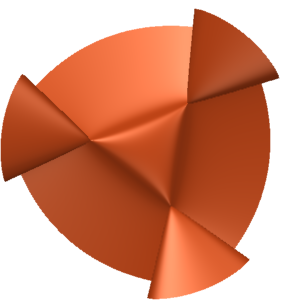
\includegraphics[width=\textwidth]{cubic3A2}
    \caption{$3A_2$}
  \end{subfigure}
  \begin{subfigure}{.24\textwidth}
    \centering
    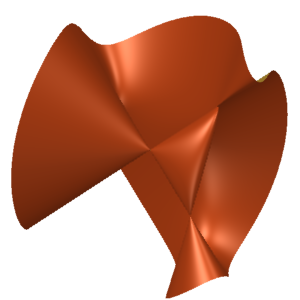
\includegraphics[width=\textwidth]{cubicA3_2A1}
    \caption{$A_3+2A_1$}
  \end{subfigure}
  \begin{subfigure}{.24\textwidth}
    \centering
    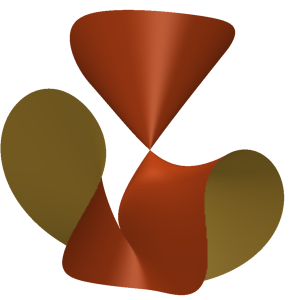
\includegraphics[width=\textwidth]{cubicA4_A1}
    \caption{$A_4+A_1$}
  \end{subfigure}
  \begin{subfigure}{.24\textwidth}
    \centering
    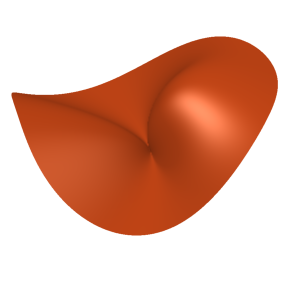
\includegraphics[width=\textwidth]{cubicD4}
    \caption{$D_4$}
  \end{subfigure}
  \caption{Some cubic surfaces with a $\G_m$-action that are not in
    the closure of the orbit of a generic cubic surface. We used the
    nice 3D grapher
    \href{https://singsurf.org/parade/Cubics.php}{here} for these
    images.}
  \label{fig:surfaces}
\end{figure}

We now the reap the benefits.
Let $X \subset \P^3$ be a cubic surface $X$ which does not lie in the closure of the orbit of a generic cubic surface.
Let $G$ be the automorphism group of $X$ and $\G_m \to G$ a one-parameter subgroup.
The family
\[ [X/\G_m] \to B\G_m\]
yields a relation
\begin{equation}\label{eqn:isorel}
  0 = a_{1^4}v_1^4 + a_{1^2\cdot 2} v_1^2v_2 + a_{1\cdot 3} v_1v_3 + a_{2^2}v_2^2 + a_4 v_4,
\end{equation}
where the $v_i$ are the Chern classes of the push-forward of the anticanonical bundle.

Let us explain how to compute the push-forward of the anti-canonical bundle.
For an integer $a$, let $\chi(a)$ denote the $1$-dimensional $\G_m$ representation where the $\G_m$ action is given by
\[ t \colon v \mapsto t^a v.\]
Suppose $X \subset \P^3$ is the zero-locus of a homogeneous cubic form $F \in k[x_0,x_1,x_2,x_3]$.
Assume that the $\G_m$ acts on the variables $x_i$ by scaling, say $t \in \G_m$ acts by
\[ t \colon x_i \mapsto t^{w_i}x_i,\]
where $w_i \in \Z$.
Since $V(F)$ is $\G_m$-fixed, there exists $w \in \Z$ such that
\[ F \left(t x_0, t x_1, t x_2, t x_3\right) = t^w F\left(x_0, x_1, x_2,x_3\right).\]
Write $V^\vee$ for the $k$-vector space $\langle x_0, x_1, x_2,x_3 \rangle$.
As a $\G_m$-representation, we have
\[ V^\vee = \chi(w_1) \oplus \chi(w_2) \oplus \chi(w_3) \otimes \chi(w_4).\]
The cubic $F$ defines a $\G_m$-invariant section of $\Sym^3 V^\vee \otimes \chi(-w)$.
Thus, we can view $X$ as the zero locus of the line bundle $\O(3) \otimes \pi^*\chi(-w)$ in the projective bundle $\pi \colon [\P V/\G_m] \to B\G_m$.
By the adjunction formula, we get
\[ \omega_X^{-1} = \O_{\P V}(1) \otimes \det V \otimes \pi^*\chi(w) |_X,\]
and hence
\begin{equation}\label{eqn:rep}
\begin{split}
  \pi_*\left( \omega_X^{-1} \right) &= V^\vee \otimes \det V \otimes \chi(w) \\
  &\cong \left( \bigoplus \chi(w_i)  \right) \otimes \chi\left(-\sum w_i\right) \otimes \chi(w).
\end{split}
\end{equation}

\subsection{The family $3A_2$}
Consider
\[ X = V(x_0x_1x_3 - x_2^3).\]
A $\G_m$ stabilizing $X$ acts on the variables by weights $(a,b,0,c)$ where $a,b,c \in \Z$ are any such that $a+b+c = 0$.
Note that in this case, the weight $w$ of the cubic equation defining $X$ is $0$.
Hence, from \eqref{eqn:rep}, we get
\[ \pi_*\left(\omega^{-1}_X\right) = \chi(a) \oplus \chi(b) \oplus \chi(0) \oplus \chi(c).\]
Letting $q = c_1(\chi(1)) \in A^1(B\G_m)$, we get
\[ v_1 = 0, \quad v_2 = (ab+bc+ca) \cdot q^2, \quad v_3 = abc \cdot q^3, \quad v_4 = 0,\]
and hence
\[ v_1^4 = 0, \quad v_1^2v_2 = 0, \quad v_1v_3 = 0,\quad v_2^2 \neq 0, \quad v_4 = 0.\]
Substituting in \eqref{eqn:isorel} yields the relation
\begin{equation}\label{eqn:iso1}
  a_{2^2} = 0.
\end{equation}

\subsection{The family $A_3 + 2A_1$}
Consider
\[ X = V(x_3(x_0x_2-x_1^2) - x_0x_1^2).\]
A $\G_m$ stabilizing $X$ acts on the variables by weights $(-3,1,5,-3)$.
The weight $w$ of the cubic equations defining $X$ is $-1$.
From \eqref{eqn:rep}, we get
\[ \pi_*\left( \omega_X^{-1} \right) = \chi(-4) \oplus \chi(0) \oplus \chi(4) \oplus \chi(-4).\]
Setting $q = c_1(\chi(1)) \in A^1(B\G_m)$, we get
\[ v_1 = -4q, \quad v_2 = -16q^2, \quad v_3 = 64q^3, \quad v_4 = 0,\]
and hence
\[ v_1^4 = 256q^4 \quad v_1^2v_2 = -256q^4, \quad v_1v_3 = -256q^4, \quad v_2^2 = 256q^4, \quad v_4 = 0.\]
Substituting in \eqref{eqn:isorel} yields the relation
\begin{equation}\label{eqn:iso2}
  a_{1^4} - a_{1^2 2}- a_{13} +  a_{2^2}  = 0.
\end{equation}

\subsection{The family $A_4 + A_1$}
Consider
\[ X = V(x_3(x_0x_2-x_1^2) - x_0^2x_1).\]
A $\G_m$ stabilizing $X$ acts on the variables by weights $(1,-1,-3,3)$.
The weight $w$ of the cubic defining $X$ is $1$.
From \eqref{eqn:rep}, we get
\[ \pi_*\left( \omega_X^{-1} \right) = \chi(2) \oplus \chi(0) \oplus \chi(-2) \oplus \chi(4).\]
Setting $q = c_1(\chi(1)) \in A^1(B\G_m)$, we get
\[ v_1 = 4q, \quad v_2 = -4q^2, \quad v_3 = -16q^3, \quad v_4 = 0,\]
and hence
\[ v_1^4 = 256q^4 \quad v_1^2v_2 = -64q^4, \quad v_1v_3 = -64q^4, \quad v_2^2 = 16q^4, \quad v_4 = 0.\]
Substituting in \eqref{eqn:isorel} yields the relation
\begin{equation}\label{eqn:iso3}
  16a_{1^4} -4a_{1^2 2}- 4a_{13} + a_{2^2}  = 0.
\end{equation}

\subsection{The family $D_4$}
Consider
\[ X = V(x_3x_0^2 - x_1^3+x_2^3).\]
A $\G_m$ stabilizing $X$ acts on the variables by weights $(5,1,1,-7)$.
The weight $w$ of the cubic equation defining $X$ is $3$.
By \eqref{eqn:rep}, we get
\[ \pi_*\left( \omega_X^{-1} \right) = \chi(8) \oplus \chi(4) \oplus \chi(4) \oplus \chi(-4).\]
Setting $q = c_1(\chi(1))$, we get
\[ v_1 = 12q, \quad v_2 = 16q^2, \quad v_3 = -192q^3, \quad v_4 = -512q^4,\]
and hence
\[ v_1^4 = 20736q^4 \quad v_1^2v_2 = 2304q^4, \quad v_1v_3 = -2304q^4, \quad v_2^2 = 256q^4, \quad v_4 = -512q^4.\]
Substituting in \eqref{eqn:isorel} yields the relation
\begin{equation}\label{eqn:iso4}
  81a_{1^4} +9a_{1^2 2}- 9a_{13} +  a_{2^2}-2a_4  = 0.
\end{equation}

\subsection{Families over a base scheme}\label{sec:schematicexample}
By choosing a suitable base $B$ and a map $B \to B \G_m$, we
can construct an isotrivial family over $B$ by pulling back one of the
families above.  We describe this explicitly in an example.

Let $B = \P^4$.  Set
\[V^\vee = \mathcal O(5) \oplus \mathcal O(1) \oplus \mathcal O(1) \oplus
  \mathcal O(-7).\] Let $x_0, x_1, x_2, x_3$ be generators of the four
summands on the standard $\A^4 \subset \P^4$.  We have
the section $(x_3x_0^2-x_1^3-x_2^3)$ of
$\Sym^3 V^\vee = \mathcal O(3)^{\oplus 20}$.  Note that this section has a
pole of order $3$ along the hyperplane at infinity.  As a result, it
defines a section $\xi$ of $\Sym^3 V^\vee \otimes \mathcal O(-3)$, which is
nowhere vanishing.  Equivalently, $\xi$ is a section of
$\mathcal O_{\P V}(3) \otimes \pi^* \mathcal O(-3)$.  Our family
$\mathcal X \to B$ is defined by the zero-locus of $\xi$ in
$\P V \to B$.

\section{The equivariant orbit class}
We use the information provided by the test families to prove the theorems advertised in the introduction.

Let $V$ be a 4 dimensional vector space.
Recall our notation $W$ for the $\GL V$ representation 
\[W = \Sym^3V^\vee \otimes \det V\]
and
\[\mathscr M = \left[ W \setminus \{0\} / \GL V \right]\]
for the moduli stack of cubic surfaces.
\begin{theorem}\label{thm:eqvclass}
  Let $X$ be a generic cubic surface.
  Then the class of $\Orb(X)$ in $A^4_{\GL V}(W) = A^4(\mathscr M)$ is given by
  \[
    [\Orb(X)] = 1080 \cdot \left(v_{1}^{2}v_{2} - v_{1}v_{3}+ 9v_{4}\right),
  \]
  where $v_i = c_i(V)$ are the Chern classes of the standard representation of $\GL V$.
\end{theorem}
\begin{proof}
  By excision and homotopy invariance of equivariant Chow groups, we have
  \[ A^4(\mathscr M) = A^4_{\GL V}(W) = A^4_{\GL V}(\bullet).\]
  The ring $A^*_{\GL V}(\bullet)$ is generated by the classes $v_i$, and hence $A^4_{\GL V}(\bullet)$ is a free $\Z$-module generated by the monomials in $v_i$ of total degree 4.
  Therefore, for every cubic surface $X$, we have an expression
  \[[\Orb(X)] = a_{1^4}v_1^4 + a_{1^2\cdot 2} v_1^2v_2 + a_{1\cdot 3} v_1v_3 + a_{2^2}v_2^2 + a_4 v_4,\]
  for some coefficients $a_i \in \Z$.
  The families in \autoref{sec:testfamilies} give the following linear relations among the coefficients
  \begin{align*}
    16 \cdot a_{1^4} + 4 \cdot a_{1^2 2} + a_{2^2} &= 4320 \text{ from \eqref{eq:relation1}}\\
    625 a_{1^{4}} + 125 a_{1^{2}2} - 25a_{13} + 25a_{2^2} - 6 a_{4} &= 103680 \text{ from \eqref{eq:relation2}}\\
    3436a_{1^4} + 1076 a_{1^{2}2} +116 a_{13} + 316 a_{2^2} &= 1036800 \text{ from \eqref{eq:relation3}}\\
    6a_{1^{4}} + 21a_{1^{2}2}+6a_{13}+16a_{2^{2}}+a_{4} &= 25920 \text{ from \eqref{eq:relationB4}}\\
    a_{2^2} &= 0  \text{ from \eqref{eqn:iso1}}\\
    a_{1^4} - a_{1^2 2}- a_{13} +  a_{2^2}  &= 0  \text{ from \eqref{eqn:iso2}}\\
    16a_{1^4} -4a_{1^2 2}- 4a_{13} +  a_{2^2}  &= 0  \text{ from \eqref{eqn:iso3}}\\
    81a_{1^4} +9a_{1^2 2}- 9a_{13} +  a_{2^2}-2a_4  &= 0  \text{ from \eqref{eqn:iso4}}.
  \end{align*}
  These equations uniquely determine all the coefficients $a_i$ to be as stated.
\end{proof}

\begin{corollary}
  The degree of the closure of the $\PGL_4$ orbit of a generic cubic surface in $\P^3$ is $96120$.
\end{corollary}
\begin{proof}
  Let $F_i$ for $i = 0,\dots,4$ be generic cubic forms in four variables.
  Consider the linear system of cubic surfaces
  \[ u_0F_0 + \dots + u_4F_4\]
  parametrized by $[u_0:\dots:u_4] \in \P^4$.
  More formally, consider the hypersurface
  \[ \mathcal X \subset \P^3 \times \P^4\]
  defined by
  \[ \mathcal X = V(u_0F_0 + \dots + u_4F_4).\]
  The second projection gives a family of cubic surfaces $\pi \colon \mathcal X \to \P^4$ and hence a map $\P^4 \to \mathscr M$.
  By adjunction, we have
  \[ \omega_\pi = \O(1) \boxtimes \O(1),\]
  and hence
  \[ \mathcal V = \pi_* \omega_\pi \cong \O(1)^{\oplus 4}.\]
  Let $S \subset \P^3$ be a cubic surface.
  By \autoref{thm:eqvclass}, if $S$ is generic, then the degree of the pull-back of $\Orb(S)$ to $\P^4$ is given by
  \[ 1080 \cdot \left(v_{1}^{2}v_{2} - v_{1}v_{3}+ 9v_{4}\right) = 96120.\]
\end{proof}

\begin{corollary}
  Let $X \subset \P^4$ be a general cubic 3-fold, and let $\pi \colon \mathcal X \to \P^4$ be the family of hyperplane sections of $X$.
  Given a generic cubic surface $S$, there are $42120$ fibers of $\pi$ isomorphic to $S$.
\end{corollary}
\begin{proof}
  Note that two cubic surfaces are isomorphic if and only if they are in the same $\PGL_4$ orbit.
  Consider the pull-back of $\Orb(S)$ to the base $\P^4$ of the family.
  By the genericity of $X$ and $S$, this pull-back consists of distinct reduced points corresponding to the points of $\Orb(S) \setminus \partial \Orb(S)$.
  The statement now follows from \autoref{thm:eqvclass} and the computation of the right hand side, which we omit.
\end{proof}

\subsection{Proof of \texorpdfstring{\autoref{theorem:main}}{first theorem} from the introduction}
%\label{proof:main}
The theorem follows immediately from \autoref{thm:eqvclass} and \autoref{prop:goodisgood}.

\subsection{Proof of \texorpdfstring{\autoref{thm:eqvclass2}}{second theorem} from the introduction}\label{proof:eqvclass2}
Let $V$ be a 4-dimensional vector space.
Set
\[\mathscr N = \left[ \Sym^3V^\vee \setminus \{0\} / \GL V \right]. \]
Let $\mathcal V$ denote the vector bundle on $\mathscr N$ corresponding to the standard representation of $\GL V$.
The tautological non-zero section of $\Sym^3V^\vee$ on $\mathscr N$ defines a family of cubic surfaces
\[ \pi \colon \mathscr X \to \mathscr N,\]
and hence a map $\mathscr N \to \mathscr M$.
Under this map, the pull-back of a generic orbit closure is a generic orbit closure.
Note that $\mathscr X \subset \P \mathcal V$ is the zero locus of $\O(3)$.
By adjunction, we have
\[ \omega_\pi = \O(1) \otimes \det V |_{\mathscr X},\]
and hence
\[ \pi_* \omega_\pi = V^\vee \otimes \det V.\]
\autoref{thm:eqvclass} gives the class of the pull-back of a generic orbit closure in terms of the Chern classes $v_i = c_i(V^\vee \otimes \det V)$.
Writing them in terms of $c_i = c_i(V)$ yields the result.

\appendix



\section{The goodness of the $A5$ cubic surface}
\label{sec:goodnessA5}

\subsection{Objective}
Let $X \subset \P^{3}$ denote the cubic surface defined in homogeneous
coordinates $\left(x_{0}, x_{1}, x_{2}, x_{3}\right)$ by the equation
\[x_{3}f_{2} - f_{3} = 0,\] where $f_{2} = x_{0}x_{1}$ and
$f_{3} = x_{0}^3 + x_{1}^{3}-x_{1}x_{2}^{2}$.  This is the unique
cubic surface possessing a single $A_5$ singularity, up to projective
equivalence.  For the reader's amusement, we include a real picture of
$X$ in \autoref{figure:cubicA5}.

\begin{figure}
  \centering
  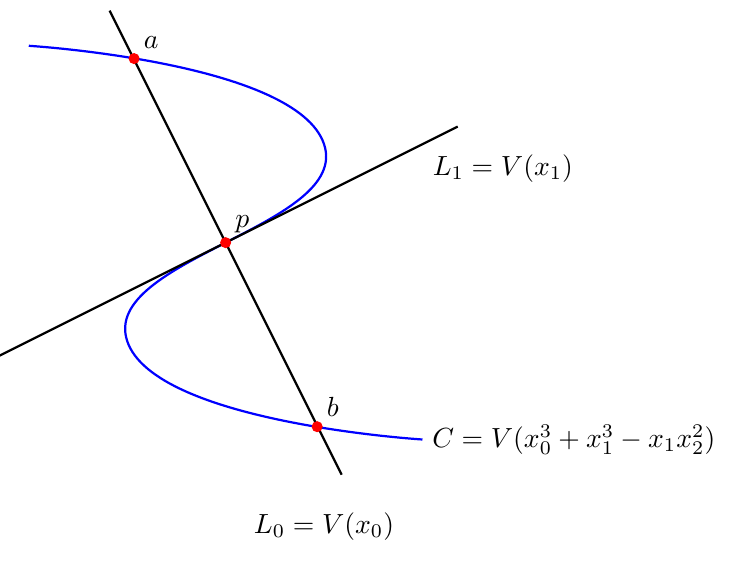
\begin{tikzpicture}[scale=1.25]
  \draw[blue, thick, smooth, tension=1] plot coordinates{
    (2,-2)
    (-1, -1)
    (1,1)
    (-2, 2)
  };
  \draw (2,-2) node [right] {$C = V(x_0^3+x_1^3-x_1x_2^2)$};
  \draw[shorten >=-0.5cm, shorten <=-0.5cm, thick] (-2,-1) -- (2,1) node [below right] {$L_1 = V(x_1)$};
  \draw[shorten >=-0.5cm, shorten <=-0.5cm, thick] (-1,2) -- (1,-2) node [below=0.8cm] {$L_0 = V(x_0)$};
  \draw[red, fill] (0,0) circle (0.05) node [black, above right] {$p$};
  \draw[red, fill] (-0.93, 1.87) circle (0.05) node [black, above right] {$a$};
  \draw[red, fill] (0.93, -1.87) circle (0.05) node [black, above right] {$b$};
\end{tikzpicture}

%%% Local Variables:
%%% mode: latex
%%% TeX-master: "../main"
%%% End:

  \caption{The surface $X$ with an $A_5$ singularity is obtained by blowing up the subscheme $a+b+4p$ in a smooth cubic $C$, where $p \in C$ is a flex point and $a, b, p$ are collinear.}
\end{figure}

\begin{figure}
  \centering
  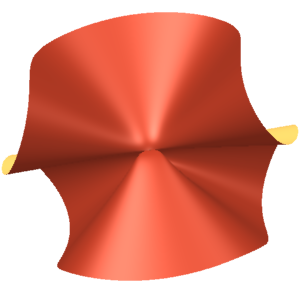
\includegraphics[width=0.25\textwidth]{cubicA5}
  \caption{The unique cubic surface $X$ with an $A_5$ singularity}
  \label{figure:cubicA5}
\end{figure}

$X$ is the cubic surface associated to the admissible length $6$
subscheme $Z \subset \P^{2}$ defined by the common vanishing of the
forms $f_{2}$ and $f_{3}$. We leave it to the reader to check that
$\Aut(\P^{2},Z)$ is one-dimensional, with $\G_{a}$ as identity
component.  Thus, the techniques used in the main body of the paper
cannot address the goodness of $X$.  The techniques developed in this
appendix likely have broader range, but we have not pursued greater
generality here in the interest of keeping the paper more focused.


Our goal is to show:

\begin{theorem}
  \label{theorem:A5good} The surface $X$ is good, i.e. $X$ does not
  lie in the $\PGL_4$-orbit closure of a general cubic surface.
\end{theorem}

The proof proceeds by contradiction, in several steps. Let
$\Delta = \spec \k [\![t]\!]$ with closed point denoted $0$ and generic
point denoted $\eta$, and suppose for sake of contradiction, that
\[\pi: \mathcal{X} \to \Delta\]
is a family of cubic surfaces with the properties:
\begin{enumerate}
\item $\mathcal{X}_{0} \simeq X$, and\\
\item $\mathcal{X}_{\eta} \simeq Y \times_{\spec \k} \eta$, where $Y$ is a
  general fixed cubic surface.
\end{enumerate}

The overall strategy is to transfer to the setting of families of
length $6$ subschemes of the plane, and reduce to proving that
$[Z] \in \Hilb^{6}\P^{2}$ does not lie in the $\PGL_3$-orbit closure
of a {\sl general} length $6$ scheme $[Z_{gen}] \in \Hilb^{6}\P^{2}$.
We will sketch several parts of the reduction, leaving lesser details
to the reader.

The following is an instance of Brieskorn's ``simultaneous resolution of singularities'', see \cite{brieskorn1970singular}:

\begin{lemma}[Brieskorn]
  \label{lemma:simult} There exists a {\sl smooth} family of cubic
  surfaces \[\pi': \mathcal{X}' \to \Delta\] and a morphism
  $\beta: \mathcal{X}' \to \mathcal{X}$ of $\Delta$-schemes which is
  an isomorphism over $\eta$ and is a minimal desingularization over
  $0$.
\end{lemma}

Let $\kappa: \Bl_{Z}\P^2 \to X$ denote the anti-canonical map. The
minimal desingularization $\beta_{0}: X' \to X$ factors through
$\kappa$, and is also the minimal desingularization of $\Bl_{Z}\P^{2}$
-- the argument for this can be found in the proof of
\autoref{prop:good}. Let $\kappa':X' \to \Bl_{Z}\P^{2} \to \P^{2}$
denote the composite map.  The line bundle
\[\mathcal{L}_{0} := \kappa'^{*}\O_{\P^{2}}(1)\] is easily seen to have
no higher cohomology, and $h^{0}(X', \mathcal{L}_{0}) = 3$.

Our next step is to extend $\mathcal{L}_{0}$ to $\mathcal{X'}$.

\begin{lemma}
  \label{lemma:extends} There exists a line bundle $\mathcal{L}$ on
  $\mathcal{X}'$ extending $\mathcal{L}_{0}$ on
  $X' \subset \mathcal{X}'$.
\end{lemma}

\begin{proof}[Proof sketch.]
  The deformation space of the pair $(X', \mathcal{L}_{0})$ is the
  cohomology group $H^1 \left( X', \mathcal{E} \right)$, where
  $\mathcal{E}$ is the extension
  \[0 \to \O_{X'} \to \mathcal{E} \to T_{X'} \to 0 \] defined by the
  element $c_{1} \mathcal{L}_{0} \in H^{1}(X', \Omega_{X'})$. Since
  $H^{2}(\O_{X'}) = 0$, it follows that $\mathcal{L}_{0}$ lifts to
   every infinitesimal deformation of $X'$.  In particular,
  $\mathcal{L}_{0}$ lifts to the formal completion of $\mathcal{X'}$
  along $X'$.  By standard algebraization arguments, we deduce a lift
  to $\mathcal{X'}$ itself.
\end{proof}

Next, we choose an isomorphism
$\P \left( \pi'_{*}(\mathcal{L})^{\smvee} \right) \simeq \P^{2}
_{\Delta}$, and let
\[\varphi: \mathcal{X}' \to \P^{2}_{\Delta}\] denote the map induced
by the line bundle $\mathcal{L}$ referenced in
\autoref{lemma:extends}.  The natural injection of line bundles
(induced by pullback of forms)
$\omega_{\mathcal{X'}/\Delta}^{-1} \hookrightarrow
\varphi^{*}\omega_{\P^{2}_{\Delta}/\Delta}^{-1}$ induces an inclusion
of free $\k[\![t]\!]$-modules
\[\pi'_{*}\left(\omega_{\mathcal{X'}/\Delta}^{-1} \right) \hookrightarrow
  H^{0}\left(\P^{2}_{\Delta}, \O(3)\right).\] The former is a rank $4$
free module, and the latter is a rank $10$ free module.  We let
\[\mathcal{Z} \subset \P^{2}_{\Delta}\] denote the closed subscheme defined by the common vanishing of the cubic forms on $\P^{2}_{\Delta}$ lying in the submodule $\pi'_{*}\left(\omega_{\mathcal{X'}/\Delta}^{-1} \right) \hookrightarrow
H^{0}\left(\P^{2}_{\Delta}, \O(3)\right)$.

Tracing through the construction fiber-by-fiber over $\Delta$, the
reader can check that $\mathcal{Z} \to \Delta$ is a finite, flat
degree $6$ cover, with central fiber $\mathcal{Z}_{0} \subset \P^{2}$
isomorphic to the admissible scheme $Z \subset \P^{2}$ from the
beginning of this appendix.  Furthermore, since the cubic surface $Y$
was chosen to be general, and since the generic fiber
$\mathcal{X'}_{\eta} \simeq \mathcal{X}_{\eta}$ is isomorphic to the
constant family $Y \times _{\spec \k} \eta$, it follows that
$\mathcal{Z}_{\eta} \subset \P^{2} \times_{\spec _{\k}} \eta$ is
isomorphic to a general, constant family of subschemes, namely, that
there exists a general length $6$ subscheme $Z_{gen} \subset \P^{2}$
and an element $g \in \Aut (\P^{2}_{\eta})$ such that
$g(Z_{gen}) = \mathcal{Z}_{\eta}$.

After performing a finite, ramified base change $t \mapsto t^{k}$, we
may assume that $\mathcal{Z} \subset \P^{2}_{\Delta}$ is the union of
$6$ sections,
$a, b, z_{1}, z_{2}, z_{3}, z_{4}: \Delta \to \P^{2}_{\Delta}$, where:
\begin{itemize}
\item $a$ and $b$ do not intersect, and
  $a(0) = [0:1:1], b(0) = [0:-1:1]$ are the two smooth points of
  $Z \subset \P^{2}$, and
\item $z_{i}(0) =[0:0:1] =: p$.
\end{itemize}
Here, we are using homogeneous coordinates $[x_0 :x_1 : x_2]$ on
$\P^{2}$ where $Z \subset \P^{2}$ is the common vanishing scheme of
$f_{2} = x_0 x_1$ and $f_3 = x_0^3+x_1^3-x_1x_2^2$.  Let
$L_{0}, L_{1} \subset \P^{2}$ denote the lines $x_0 = 0$ and $x_1=0$,
respectively. The line $L_0$ contains the three points supporting $Z$, while
$L_1$ is the tangent line of $Z$ at its multiplicity $4$ point $p$.


\subsection{Resolving rational maps $\P^{2}_{\Delta} \dashrightarrow \P^{2}_{\Delta}$}
\label{sec:resolv-rati-maps}

Maintaining the notation above, we have arrived at the following
situation:
\begin{enumerate}
\item $Z_{gen} \subset \P^{2}$ is a general set of $6$ points, denoted $q_{1}, q_{2}, p_{1}, p_{2}, \dots, p_{4}$,\\
\item A rational map
  $g : \P^{2}_{\Delta} \dashrightarrow \P^{2}_{\Delta}$ restricting to
  an element of $\Aut \P^{2}_{\eta}$ over the generic point $\eta$, \\
\item The Zariski closure
  $\overline{g(Z_{gen} \times_{\spec \k} \eta)}$ is
  $\mathcal{Z} \subset \P^{2}_{\Delta}$.  We assume that
  $q_{1}, q_{2}$ map to $a,b$ correspondingly, and that $p_{i}$ maps
  to $z_{i}$.
\end{enumerate}

The strategy then to show that this situation is impossible.  For
this, we need to study the basic anatomy of a rational map
\[g: \P^{2}_{\Delta} \dashrightarrow \P^{2}_{\Delta} \] induced by an
element of $\Aut \P^{2}_{\eta}$.

Letting $[x_0 : x_1 : x_2]$ denote homogeneous coorinates on $\P^{2}$,
the rational map $g$ is given by $3$ homogeneous linear forms
$A_0, A_1, A_2 \in \k(\!(t)\!)[x_0,x_{1},x_{2}]$.  By multpilying by a
suitable power of $t$, (not affecting the map $g$), we may assume that
$A_{i} \in \k[\![t]\!][x_0, x_1, x_2]$, and that not all $A_i$ vanish
modulo $(t)$.  Furthermore, by swapping $A_{i}$ by suitable
$\k$-linear combinations, we may assume that
$V(A_{i}) \subset \P^{2}_{\Delta}$ is an irreducible (hence smooth in
this case) divisor for all $i$.  Let $\Lambda_{i}$ denote the
subscheme $V(A_{i})$; $\Lambda_{i}$ restricts to a line over each
point of $\Delta$.


The resolution of the rational map $g$ proceeds in two stages.  First,
suppose all three divisors $\Lambda_{i}$ intersect along a line
$\lambda \subset \P^{2}_{0}$ in the fiber over $0 \in \Delta$.  We
blow up the line $\lambda$ to obtain
\[ \beta_{1}: \P^{2}_{\Delta}\left(1 \right) :=
  \Bl_{\lambda}\P^{2}_{\Delta} \to \P^{2}_{\Delta}\]

The fiber over $0 \in \Delta$ in $\P^{2}_{\Delta}(1)$ is the
transverse union of
\begin{enumerate}
\item $P$: the proper transform of $\P^{2}_{0}$, and\\
\item $F(1)$: a surface isomorphic to the Hirzebruch surface $\F_{1}$,
\end{enumerate}
where $P$ intersects $F(1)$ along $\lambda \subset P$.  On $F(1)$,
$\lambda$ is the directrix. Furthermore, $F(1)$ is the exceptional
divisor of $\beta_{1}$.  If we let $\Lambda_{i}(1)$ denote the proper
transforms of $\Lambda_{i}$, then the reader can check that
$\Lambda_{i}(1)$ are all smooth, and that $\Lambda_{i}(1)\big|_{0}$ is
a line in $F(1)$ for all $i$.  (By a {\sl line} in $\F_{1}$ we mean
the preimage of a line under the blowdown map $\F_{1} \to \P^{2}$.)

Next, suppose $\Lambda_{i}(1)$, $i=1,2,3,$ all intersect along a
particular line $\lambda(1) \subset F(1)$. Note that $\lambda(1)$ is
disjoint from the directrix $\lambda \subset F(1)$.  We can once again
blow up $\lambda(1) \subset \P^{2}_{\Delta}(1)$ to obtain
\[\beta_{2}: \P^{2}_{\Delta}(2) \to \P^{2}_{\Delta}(1).\]

The fiber over $0 \in \Delta$ in $\P^{2}_{\Delta}(2)$ is a chain of
three surfaces
\begin{enumerate}
\item $P(0)$: the proper transform of $\P^{2}_{0}$, and\\
\item $F(1)$: a surface isomorphic to the Hirzebruch surface $\F_{1}$, and\\
\item $F(2)$: another copy of $\F_{1}$, 
\end{enumerate}
where $P(0) \cup F(1)$ is the proper transform of the same named
surfaces in $\P^{2}_{\Delta}(1)$, and $F(2)$ meets $F(1)$ along
$\lambda(1)$, where $\lambda(1)$ is the directrix of
$F(2)$. Similarly, we let $\Lambda_{i}(2)$ denote the strict
transforms of $\Lambda_{i}(1)$; the surfaces $\Lambda_{i}(2)$
intersect $F(2)$ along lines which avoid the directrix.

Proceeding in this manner, we end up with the scheme
$\P^{2}_{\Delta}(n)$, whose fiber over $0 \in \Delta$ is an
``accordion'' of surfaces $P \cup F(1) \cup \dots \cup F(n)$, {\sl and
  such that the three smooth surfaces $\Lambda_{i}(n)$ now only
  intersect at a point $x \in F(n)$ not lying on the directrix of
  $F(n)$.}

\begin{figure}
  \centering
  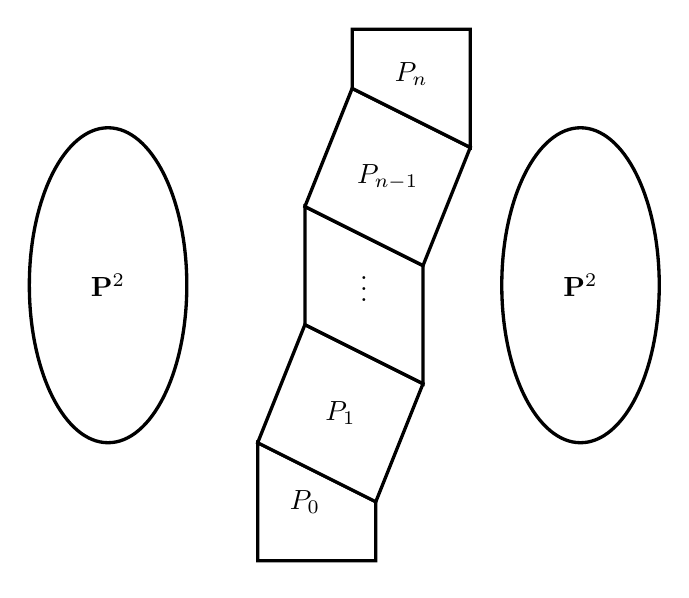
\begin{tikzpicture}[very thick]
  \begin{scope}[xshift=-3cm]
    \draw (0,0) ellipse (1 and 2);
    \draw (0,0) node {$\P^2$};
  \end{scope}
  \begin{scope}[yshift=-2cm, xshift=-0.5cm, yscale=0.75, xscale=1.5]
    \draw[fill=white] (-0.4,-2.0) -- (0.6,-2.0) -- (0.6, -1) -- (-0.4,0) -- cycle;
    \draw[fill=white] (0.6, -1) -- (-0.4,0) -- (0, 2) -- (1,1) -- cycle;
    \draw[fill=white] (0, 2) -- (1,1) -- (1,3) -- (0,4) -- cycle;
    \draw[fill=white] (1, 3) -- (0,4) -- (0.4, 6) -- (1.4,5) -- cycle;
    \draw[fill=white] (0.4, 6) -- (1.4,5) -- (1.4,7) -- (0.4,7) -- cycle;
    \draw
    (0,-1.0) node {$P_0$}
    (0.3,0.5) node {$P_1$}
    (0.5, 2.75) node {$\vdots$}
    (0.7, 4.5) node {$P_{n-1}$}
    (0.9, 6.25) node {$P_{n}$};
    \draw (0,-2) node (X) {};
  \end{scope}
  \begin{scope}[xshift=+3cm]
    \draw (0,0) ellipse (1 and 2);
    \draw (0,0) node {$\P^2$};
  \end{scope}
\end{tikzpicture}
%%% Local Variables:
%%% mode: latex
%%% TeX-master: "../main"
%%% End:

  \caption{A family of surfaces with an accordion like central fiber arises while resolving the rational map $\P^2_\Delta \dashrightarrow \P^2_\Delta$.}
\end{figure}

Thus, the rational map
$g \circ \beta_{1} \circ \dots \circ \beta_{n}: \P^{2}_{\Delta}(n)
\dashrightarrow \P^{2}_{\Delta}$ now has indeterminacy scheme
$B = \cap_{i} \Lambda_{i}(n)$ supported at the single point
$x \in F(n)$.  Note that $B$ is now a global complete intersection
subscheme of $\P^{2}(n)$, being the intersection of the three surfaces
$\Lambda_{i}(n)$. If we finally let
\[\td{\P^{2}_{\Delta}(n)}\]
denote the blow up $\Bl_{B}\P^{2}_{\Delta}(n)$, with blowdown map
denoted $\beta: \td{\P^{2}_{\Delta}(n)} \to \P^{2}_{\Delta}(n)$, we
obtain the resolution of indeterminacy $\td{g}$ of the original map
$g$:
\begin{center}
  \begin{tikzcd} & \td{\P^{2}_{\Delta}(n)} \arrow[dl] \arrow[dr, "\td{g}"]  & & \\
    \P^{2}_{\Delta} \arrow[rr, dashed, "g"] & & \P^{2}_{\Delta}
  \end{tikzcd}
\end{center}
Let $P(\infty) = \beta^{-1}(x) \subset \td{\P^{2}_{\Delta}(n)}$ denote
the exceptional surface; $P(\infty)$ is isomorphic to $\P^{2}$ because
$B$ is a complete intersection.

The map $\td{g}$ has the following effect on the fiber
$P(0) \cup F(1) \cup \dots \cup F(n-1) \cup \Bl_{x}F(n) \cup
P(\infty)$:
\begin{enumerate}
\item $\td{g}\big|_{P(\infty)}: \P(\infty) \to \P^{2}_{0}$ is an
  isomorphism \\
\item $\td{g}\big|_{\Bl_{x}F(n)}: \Bl_{x}F(n) \to \P^{2}_{0}$ is
  ``projection from the point $x$'', if we think of $F(n)$ as the blow
  up of a plane at a point not equal to $x$.  The $\td{g}$-image of
  $\Bl_{x}F(n)$ is a line $\lambda' \subset \P^{2}_{0}$.\\
\item $\td{g}$ contracts $P(0) \cup \dots \cup F(n-1)$ to a single
  point on the line $\lambda'$.
\end{enumerate}

\subsection{Finishing the argument}
\label{sec:finishargument}

Now we are in a position to finish the proof of
\autoref{theorem:A5good}.  Given what happened in the last section, we
must show that the constant subscheme
$Z_{gen} \times \Delta \subset \P^{2}_{\Delta}$ cannot transform into
$\mathcal{Z}$ under $g$.  To help the reader focus, we state from the
outset the fundamental detail ultimately obstructing this possibility:
The line $L_0$ containing the support $\{[0:1:1], [0:-1:1], [0:0:1]\}$
of $Z$ is {\sl distinct} from the line $L_1$ which is the tangent line
of $Z$ at $[0:0:1] \in Z$.

\begin{proof}[Proof of \autoref{theorem:A5good}]
  We assume the existence of a rational map $g$ under which
  $Z_{gen} \times \Delta$ transforms into $\mathcal{Z}$, and will
  eventually arrive at a contradiction.  We recall that
  $Z_{gen} = \{q_1, q_2, p_1, \dots, p_4\}$.

  First, note that in the resolution of $g$, we {\sl must} begin with
  blowing up a line $\lambda$. In fact, we must blow up the line
  $\lambda = \langle q_{1}, q_{2} \rangle \subset \P^{2}_{0}$.  If we
  did not do so, then by the description of the resolution $\td{g}$
  given at the end of \autoref{sec:resolv-rati-maps}, at least one of
  the two points $q_{i}$ would become identified with the four points
  $p_{j}$ under $\td{g}$ in the fiber over $0 \in \Delta$, contrary to
  the nature of $Z$.

  Next, we claim that in the resolution of $g$, in the final step,
  there {\sl must} be a finite, non-empty base point $x \in F(n)$ as
  described in the general resolution process in
  \autoref{sec:resolv-rati-maps}.  If not, then $\td{g}\big|_{F(n)}$
  would be the contraction of the Hirzebruch surface $F(n)$ down to
  $\P^{2}_{0}$.  By the reasoning in the previous paragraph, the
  proper transforms of the sections $\{q_{i}\} \times \Delta$ in
  $\P^{2}_{\Delta}(n)$ must meet $F(n)$ in a pair of points
  $\td{q}_{i}$ outside the directrix of $F(n)$ while the proper
  transforms of $\{p_{j}\} \times \Delta$ must lie in
  $P(0)$. Furthermore, the line
  $\langle \td{q}_{1}, \td{q}_{2} \rangle \subset F(n)$ must be
  disjoint from the directrix, because otherwise the pair $\td{q}_{i}$
  would be identified under the blow-down map to the domain
  $\P^{2}_{\Delta}$, which is obviously not the case.  Thus, if there
  were no further basepoint $x$ to resolve in $F(n)$, the
  $\td{g}$-images of the pair $\td{q}_{i}$ would span a line which
  does not contain the point $p \in Z$, again contrary to the nature
  of $Z$.

  Thus, the map $g$ would need to be resolved by blowing up a finite
  scheme $B \subset \P^{2}_{\Delta}(n)$ meeting $F(n)$ at a point $x$,
  as described in \autoref{sec:resolv-rati-maps}. In our current
  situation, the surface $F(n)$ contains the pair of points
  $\td{q}_{i}$ and also the basepoint $x$, which may or may not
  coincide with one of the $\td{q_{i}}$.  In any case, since the
  effect of $\td{g}$ on $F(n)$ is ``projection away from $x$'', we
  deduce that the image of $F(n)$ must be the line
  $L_0 \subset \P^{2}_{0}$ joining $a$ or $b$ with $p$.  Our proof
  will be complete after we contradict this conclusion.

  
  To continue, we let $\Sigma_{j,k}$ denote the irreducible surface in
  $\P^{2}_{\Delta}(n)$ obtained by taking the closure of the line
  $\langle \{p_{j}\} \times \eta, \{p_{k}\} \times \eta \rangle$
  defined over the generic point $\eta$.  Let
  $C_{j,k} \subset P(0) \cup \dots \cup F(n)$ denote the fiber of
  $\Sigma_{j,k}$ over $0 \in \Delta$. $C_{j,k}$ is a chain of
  $\P^{1}$'s, with $C_{j,k} \cap P(0)$ being the line joining
  $p_{j}, p_{k}$ viewed as points in $P(0)$. The curves
  $C_{j,k} \cap F(m)$, varying across all choices of $j,k$ are then
  ruling lines which are uniquely determined by the locations of the
  points
  $\langle q_{1}, q_{2} \rangle \cap \langle p_{j}, p_{k} \rangle$,
  which in turn (using the generality of $Z_{gen}$) is a set of $6$
  distinct points.  In particular, $x \notin C_{j,k}$ for some pair
  $j,k$.  This implies that $\td{g}(C_{j,k})$ =
  $L_{0} \subset \P^{2}_{0}$.  However, $\td{g}(C_{j,k})$ must {\sl
    also} be the limit of the line joining the pair of sections
  $z_{j}, z_{k} \subset \mathcal{Z}$ over the generic point $\eta$.
  This latter line is $L_{1}$, which is distinct from $L_0$, providing
  our desired contradition.
\end{proof}




\bibliographystyle{plain}
\bibliography{references.bib}
\end{document}

%%% Local Variables:
%%% mode: latex
%%% TeX-master: t
%%% End:



